\documentclass[10pt]{article}
\usepackage[margin=1in]{geometry}
\usepackage{jheppub} % for details on the use of the package, please see the JINST-author-manual
% page formatting
\usepackage{fancyhdr}
\pagestyle{fancy}

\renewcommand{\sectionmark}[1]{\markright{\textsf{#1}}}
\renewcommand{\subsectionmark}[1]{}
\lhead{\textbf{\thepage} \ \ \nouppercase{\rightmark}}
\chead{}
\rhead{}
\lfoot{}
\cfoot{}
\rfoot{}
\setlength{\headheight}{14pt}

\linespread{1.03} % give a little extra room
\setlength{\parindent}{0.2in} % reduce paragraph indent a bit
\setcounter{secnumdepth}{2} % no numbered subsubsections
\setcounter{tocdepth}{2} % no subsubsections in ToC

\usepackage{lineno}
\usepackage{amsmath,amsthm,amsfonts,amssymb,amscd,physics,cancel,mathtools}
\usepackage{tcolorbox}
\usepackage{marginnote,tensor}
\usepackage[spanish]{babel}
%~~~~~~~~~ Document setup
% \usepackage[spanish]{babel} % English formatting
\usepackage[utf8]{inputenc} % Standard encoding
% \usepackage[a4paper,left=3cm,bottom=3cm]{geometry} % Page formatting
\usepackage{indentfirst} % Indents the first paragraph
\usepackage{amsmath} % Maths type package
\usepackage{bm} % Bold font maths
\usepackage{graphicx} % Advanced graphics package
\usepackage[export]{adjustbox} 
\usepackage{pdflscape} % Make pages landscape
\usepackage{fancyhdr} % Fancy headers
% \usepackage[colorlinks=true,citecolor=blue,urlcolor=blue,linkcolor=black]{hyperref} % Link colours
%\usepackage{natbib} % Bibliography
% \usepackage{flafter} % Reference any 'float'
% \usepackage[framemethod=tikz]{mdframed} % Box off stuff
\usepackage{color} % Colour support
\usepackage{wrapfig} % Text flowing around figures
\usepackage{lipsum} % Generates meaningless text
\usepackage{xcolor}
%\usepackage{biblatex}
%\usepackage[backend=bibtex]{biblatex}
%\addbibresource{bibliography.bib}
%\hypersetup{colorlinks=true, linkcolor=blue}


\theoremstyle{definition}
\newtheorem{ej}{Ejemplo}[section]
\newtheorem{sol}{Solución}[section]
\newtheorem{prop}{Propiedad}[section]
\newtheorem{dem}{Proof}[section]
\newtheorem{defi}{Definición}[section]
\newtheorem{teor}{Teorema}[section]
\newtheorem{prueba}{Prueba}[section]
\newtheorem{obs}{Observación}[section]


\newcommand{\Lag}{L=L(q_i,\dot{q}_i,t)}
\def\anillo{$(A,+,\cdot)$}
\def\campo{$(K,+,\cdot)$}
\def\espvec{$(M,K,\bullet)$}
\def\algebra{$(A,K,\bullet)$}
\def\qp{q'}
\def\tp{t'}
\def\qd{\dot{q}}
\def\qdd{\ddot{q}}
\def\qdp{\dot{q}'}
\def\dttp{\dv{t}{t'}}
\def\dtpt{\dv{t'}{t}}
\def\db{\bar{\delta}}
\def\l({\left(}
\def\r){\right)}
\def\EL{\pdv{L}{q_i}-\dv{t}\pdv{L}{\qd_i}}
\def\uin{u(x)_{i\nu}}
\def\he{\hat{e}}
\def\M{\mathcal{M}}
\def\vec{\vb*}
\def\Lmn{\Lambda^\m_{~\n }}
\def\omn{\omega^\m_{~\n }}
\def\id{\mathbb{I}}


\def\a{\alpha}
\def\b{\beta}
\def\g{\gamma}
\def\G{\Gamma}
\def\d{\delta}
%\def\D{\Delta}
%\def\e{\eta}
\def\la{\lambda}
\def\La{\Lambda}
\def\k{\kappa}
\def\m{\mu}
\def\n{\nu}
%\def\r{\rho}
\def\p{\rho}
\def\o{\omega}
\def\s{\sigma}
\def\S{\Sigma}
\def\t{\tau}
\def\p{\pi}
\def\f{\phi}
\def\vf{\varphi}
\def\ep{\epsilon}
\def\th{\theta}
\def\Th{\Theta}
\def\z{\zeta}

%-----COLORS LIST ------
\definecolor{azure(colorwheel)}{rgb}{0.0, 0.5, 1.0}
\definecolor{DarkViolet}{RGB}{148,0,211}
\definecolor{myDarkBlue}{rgb}{0,0.1,0.7}
\definecolor{DarkBlue}{RGB}{0,0,153}
\definecolor{amber}{rgb}{1.0, 0.49, 0.0}
\definecolor{amaranth}{rgb}{0.9, 0.17, 0.31}
\definecolor{nicered}{rgb}{0.7,0.1,0.1}
\definecolor{brown}{rgb}{0.5,0.1,0.1}
\definecolor{nicegreen}{rgb}{0.0,0.3,0.0}
\definecolor{tealgreen}{rgb}{0.0, 0.51, 0.5}
\def\red#1{{\color{red} #1}}
\def\green#1{{\color{green} #1}}
\def\blue#1{{\color{blue} #1}}
\def\orange#1{{\color{orange} #1}}
%----------------------
\newcommand{\mycolor}{DarkViolet}
\def\myColor#1{{\color{\mycolor} #1}}
\definecolor{tclr}{RGB}{148,0,211}
%----------------------
\newcommand{\corr}[1]{\textcolor{nicered}{#1}}
\newcommand{\nick}[1]{\textcolor{olive}{#1}}
\newcommand{\teo}[1]{\textcolor{azure(colorwheel)}{#1}}
\newcommand{\chteo}[2]{\corr{\st{#1}} \teo{(#2)}}
\newcommand{\bako}[1]{\textcolor{DarkViolet}{#1}}
\newcommand{\than}[1]{\textcolor{magenta}{#1}}

%----------------------
\usepackage{hyperref}
\hypersetup{colorlinks,bookmarksopen,
	bookmarksnumbered,
	citecolor={nicered},
	linkcolor={myDarkBlue},
	urlcolor={tealgreen},
	pdfstartview=FitH}




% \arxivnumber{1234.56789} % if you have one

%\title{\boldmath Teoría Clásica de Campos}

% Collaborations

%% [A] If main author
%% \collaboration{\includegraphics[height=17mm]{collabroation-logo}\\[6pt]
%%  XXX collaboration}

%% or
%% [B] If "on behalf of"
%% \collaboration[c]{on behalf of XXX collaboration}


% Authors
% The "\note" macro will give a warning: "Ignoring empty anchor...", you can safely ignore it.

%% [A] simple case: 2 authors, same institution
%% \author[1]{A. Uthor\note{Corresponding author.}}
%% \author{and A. Nother Author}
%% \affiliation{Institution,\\Address, Country}

%% or, e.g.
%% [B] more complex case: 4 authors, 3 institutions, 2 footnotes
%% \author[a,b]{F. Irst,\note{Now at another university}}
%% \author[c]{S. Econd,}
%% \author[a,2]{T. Hird\note{Also at Some University.}}
%% \author[c,2]{and Fourth}
%% \affiliation[a]{Institution_1,\\Address, Country}
%% \affiliation[b]{Institution_2,\\Address, Country}
%% \affiliation[c]{Institution_3,\\Address, Country}

%\author{Borja Diez}
%\affiliation{Universidad Arturo Prat}
%% \affiliation{Another University,\\
%% different-address, Country}
%
%% E-mail addresses: only for the corresponding author
%\emailAdd{borjadiez1014@gmail.com}
%
%\abstract{Estas notas son una suerte de recopilado de las clases Teoría Clásica de Campos dictadas por el Dr. Patricio Salgado el primer semestre del 2024.}




\begin{document}
% make title page
\thispagestyle{empty}
\bigskip \
\vspace{0.1cm}

\begin{center}
{\fontsize{22}{22} \selectfont Notas de Clase en}
\vskip 16pt
{\fontsize{36}{36} \selectfont \bf \sffamily Teoría Clásica de Campos}
\vskip 24pt
{\fontsize{18}{18} \selectfont \rmfamily Borja Diez} 
\vskip 6pt
{\fontsize{14}{14} \selectfont \ttfamily borjadiez1014@gmail.com}
\vskip 24pt
\end{center}

Estas notas de clase están basadas en el curso dictado por el Dr. Patricio Salgado durante el primer semestre del año 2024 en la Universidad Arturo Prat y han sido escritas con propósito de estudio personal.

Las notas están divididas por clase. Adicionalmente han sido complementadas con desarrollos de cálculo personal y comentarios sacados de la bibliografía citada al final de este documento. 

% make table of contents
\newpage
\tableofcontents
\newpage

\part{Mecánica Clásica}
\section{Clase 1}
\subsection{Mecánica de Newton}
Posición, velocidad, aceleración, fuerza.

Si consideramos un sistema de partículas de masa $m$
\begin{equation}
  \vec{p}_\alpha =m_\alpha \vec{\dot{x}}_\alpha,\qquad \vec{p}=\sum_\alpha \vec{p}_\alpha,\qquad \alpha=1,...,k
\end{equation}
\begin{equation}
  T=\frac{1}{2}\sum_\alpha m_\alpha \vec{\dot{x}}^2,\qquad \vec{L}=\sum_\alpha \vec{x}_\alpha\times \vec{p}_\alpha
\end{equation}
Newton estableció que a dinámica de un sistema mecánico queda	determinada por tres leyes fundamentales:
\begin{itemize}
	\item \textbf{Primera ley del movimiento:} Todo cuerpo en reposo permanecerá en reposo o en movimiento rectilíneo uniforme (MRU), a menos que una fuerza externa actúe sobre él.
	\item \textbf{Primera ley del movimiento:} Un cuerpo cambia su estado de movimiento si una fuerza actúa sobre él
	\begin{equation}
  \vec{F}=m\vec{a}
\end{equation}

\item \textbf{Tercera ley del movimiento:} A cada acción le corresponde una reacción paralela y opuesta.
\end{itemize}

Estas lees sólo son válidas en un sistema de referencia inercial (SRI). Dos SRI están relacionados por medio de una transformación de Galileo.

\begin{figure}[h!]
	\centering
	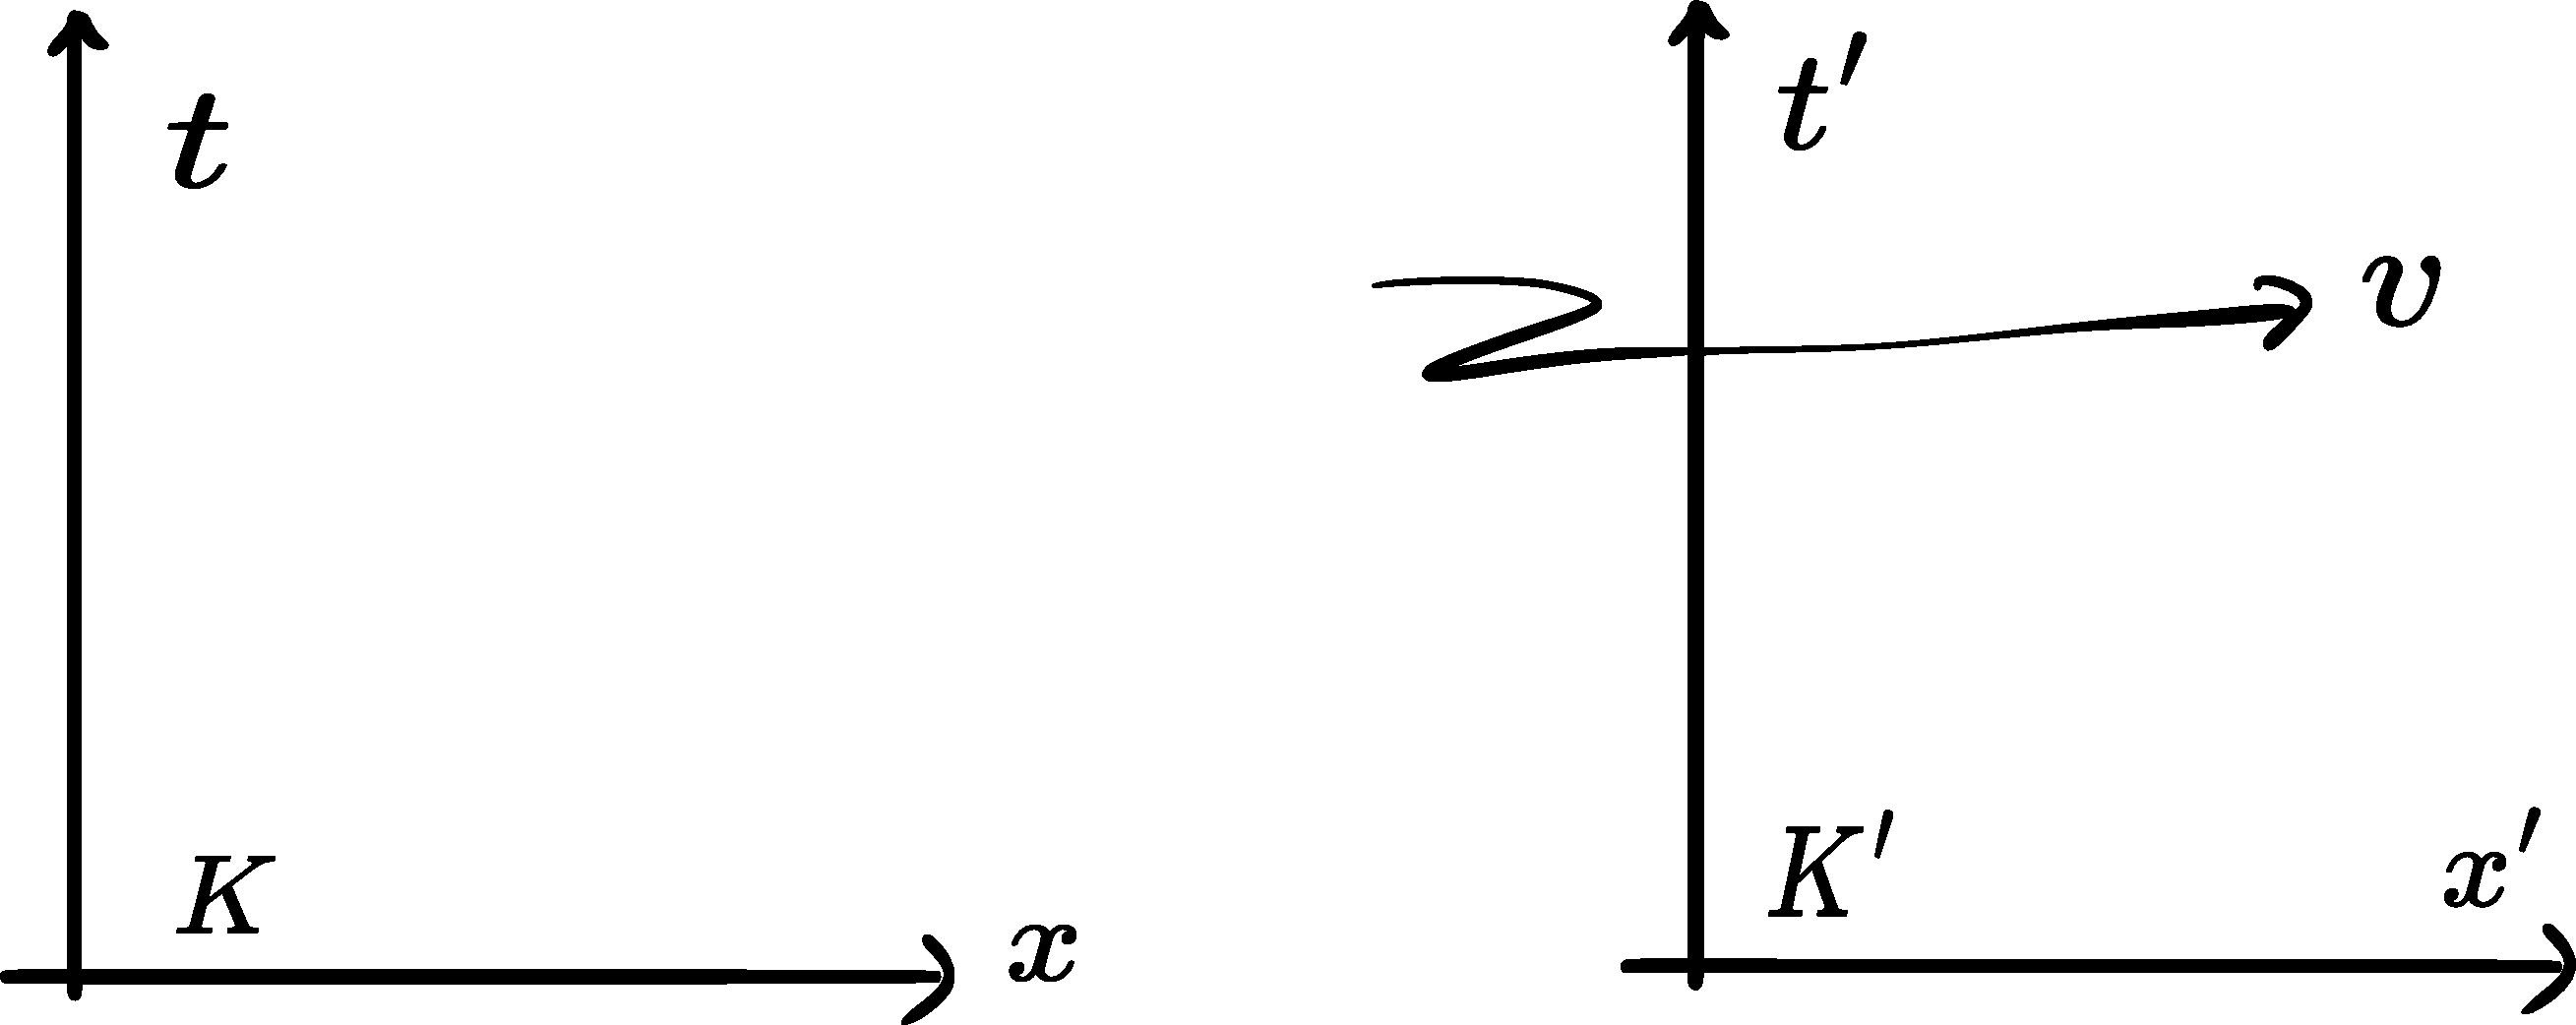
\includegraphics[scale=0.2]{fig/Galileo.pdf}
\end{figure}

\begin{align}
  x'&=x-vt\\
  t'&=t
\end{align}

Además
\begin{align}
  \vec{F}_\a &=m\ddot{\vec{x}}
\end{align}
\begin{equation}
	\implies m\ddot{\vec{x}}_\a =\dv{t}(m\dot{\vec{x}}_\a )=\dv{t}\vec{p}_\a =\dot{\vec{p}}_\a 
\end{equation}
Si las fuerzas son conservativas, se tiene
\begin{equation}
  \vec{F}_\a =-\vec{\nabla} V_\a 
\end{equation}
\begin{equation}
  \implies \boxed{\vec{\dot{p}}_\a +\vec{\nabla}V_\a =0}
\end{equation}

\subsection{Mecánica de Lagrange}
Es basada en la llamada función de Lagrange, definida como
\begin{equation}
  L(\vec{x}_\a ,\dot{\vec{x}}_\a ,t)=T(\dot{\vec{x}}_\a ,t)-V(\vec{x}_\a ,t)
\end{equation}
Lagrange introdujo el concepto de coordenada generalizada
\begin{equation}
  q_i,\quad i=1,2,...,f
\end{equation}
donde $f$ son los grados de libertad del sistema. De esta manera, se define la derivada de Euler-Lagrange como
\begin{equation}
  [L]_i=\EL=0
\end{equation}
Así, las soluciones a estas ecuaciones describen la dinámica del sistema en un espacio $f$-dimensional de coordenadas $q_i,q_2,...,q_f$.

\underline{\textbf{Nota}}: La energía cinética debe ser una función homogénea de grados dos
\begin{equation}
  T=\sum_{i,k} a_{ik}\qd_i\qd_k
\end{equation}

Notemos que una función de Lagrange dada por
\begin{equation}
  L'=L+\dv{t}B(q,t)
\end{equation}
conduce a las mismas ecuaciones del movimiento.

La libertad en la elección de coordenadas generalizadas implica que las ecuaciones de movimiento de Euler-Lagrange son \textit{estructuralmente invariantes} bajo una transofrmación de coordenadas generalizadas, es decir, bajo
\begin{equation}
  q_i\to q'_i=q'_i(q_l)\implies \qd '_i=\pdv{q'_i}{q_l}\qd_l
\end{equation}
\begin{equation}
  \pdv{\qd'_i}{\qd _l}=\pdv{q'_i}{q_l}
\end{equation}
Definiendo 
\begin{equation}
  \varphi(q_l)=\pdv{q'_i}{q_l}
\end{equation}
se tiene
\begin{equation}
  \dv{t}\varphi(q_l)=\pdv{\varphi}{q_l}\dot{q}_l
\end{equation}
luego
\begin{equation}
  \dv{t}\pdv{q'_i}{q_l}=\pdv{q_k}\left(\pdv{q'_i}{q_l}\right)\qd_k
\end{equation}
\begin{equation}\label{1.1}
  \implies \boxed{\dv{t}\pdv{q'_i}{q_l}=\pdv{q'_i}{q_k}{q_l}\qd_k}
\end{equation}
Dado que
\begin{equation}
  \qd'_i=\pdv{q'_i}{q_l}\qd_i
\end{equation}
\begin{equation}\label{1.2}
  \pdv{\qd_i}{q_l}=\pdv{q_l}\left(\pdv{\qd_i}{q_k}\qd_k\right)=\pdv{\qd_i}{q_l}{q_k}\qd_k+\cancelto{0}{\pdv{\qd_i}{q_k}\pdv{\qd_k}{q_l}}
\end{equation}
\begin{equation}
  \implies \boxed{\dv{t}\pdv{q'_i}{q_l}=\pdv{\qd_i}{q_l}}
\end{equation}
Dado que $L'(q',\qd',t)=L(q,\qd,t)$, calculemos
\begin{equation}
  \dv{t}\pdv{L'}{\qd'_k}
\end{equation}























\subsection{Acerca de la matriz Hessiana de las ecuaciones de Euler-Lagrange}
\begin{equation}
  \dv{t}\pdv{L'}{\dot{q}'_k}=\pdv{L'}{q'_k}-[L]_k\pdv{q_l}{\dot{q}_k}
\end{equation}
\begin{equation}
  \Rightarrow \pdv{L'}{q'_k}=\dv{t}\pdv{L'}{\dot{q}_k}=[L]_l\pdv	{q_l}{q'_k}
\end{equation}
\begin{equation}
\boxed{[L']_k=[L]_l\pdv{q_l}{q'_k}}
\end{equation}
La derivada de Euler-Lagrange transforma como un vector covariante bajo una transformación de coordenadas
\begin{equation}
  \mbox{Si }[L]_l=0 \Rightarrow [L']_k=0
\end{equation}



\newpage
\section{Clase 2}
\begin{enumerate}
	\item Las ecuaciones de Newton son invariantes en forma bajo las transformaciones de Galileo.
	\item Las ecuaciones de Newton sn ecuaciones de segundo orden en $\vb*{x}_\alpha$. Es bueno recalcar que \textit{todas las ecuaciones dinámicas de la física fundamental son de segundo orden}. Las ecuaciones de orden mayor al segundo, tienden a tener inestabilidades \cite{Ostrogradsky:1850fid}.
	\item Si $L=L(q_i,\dot{q}_i,t)$ es la función de Lagrange para un sistema mecánico, entonces la dinámica del sistema es gobernada por las ecuaciones de Euler-Lagrange,
	\begin{equation}\label{eqs EL}
  [L]_i=\pdv{L}{q_i}-\dv{t}\pdv{L}{\dot{q}_i}=0
\end{equation}
Estas ecuaciones no cambian si la función de Lagrange es modificada a la forma
\begin{equation}
  \tilde{L}=L+\dv{t}B(q,t)
\end{equation}
con $L=L(q_i,\dot{q}_i,t)$ y $\bar{L}=\bar{L}(q_i,\dot{q}_i,t)$
\item La libertad en la elección de las coordenadas generalizadas implica que las ecuaciones de Euler-Lagrange son estructuralmente invariantes bajo un cambio de coordenadas:
\begin{equation}\label{2.1}
  q_i\to q'_i=q'_i(q_l)
\end{equation}
lo cual implica que
\begin{equation}
  \boxed{[L']_k=[L]_l\pdv{q_l}{q'_k}}
\end{equation}
que muestra que la derivada de Euler transforma como un vector covariante bajo la transformación \ref{2.1}
\end{enumerate}
\begin{equation}
  \mbox{Si }[L]_l=0 \Rightarrow [L']_k=0.
\end{equation}

Es importante recalcar que la invariancia estructural es distinto a la invariancia en forma (covariancia).

\textit{Todos los observadores observan la misma forma de las ecuaciones de los modelos de la naturaleza.}

\begin{ej}
	La ecuación de Newton en el SRI K toma la forma $\vb*{F}=m\vb*{a}$ mientras que en el SRI $K'$ toma la forma $\vb*{F'}=m'\vb*{a}'$.
\end{ej}
\begin{ej}
	Las ecuaciones de Maxwell tendrán la misma forma en todos los SRI.
\end{ej}

Notemos son embargo, que en la mecánica de Newton las transformaciones son las transformaciones de Galileo y que en la electrodinámica de Maxwell son las transformaciones de Lorentz.

La covariancia de las ecuaciones del movimiento bajo una transformación de coordenadas es la propiedad que define una \textbf{simetría de Lie}.

\subsection{Acerca de la matriz Hessiana}
Una característica básica de las ecuaciones de Newton $m\ddot{\vb*{r}}=\vb*{F}(\vb*{r},\dot{\vb*{r}},t)$ es que es posible expresar la aceleración $\ddot{\vb*{r}}$ en función de la posición $\vb*{r}$, de la velocidad $\dot{\vb*{r}}$ y de $t$,
\begin{equation}
  \ddot{\vb*{r}}(t)=\frac{1}{m}\vb*{F}(\vb*{r},\dot{\vb*{r}}(t))
\end{equation}
Esta es una formulación vectorial de la mecánica  es basada en el concepto d partícula material. Esto llevó a pensar que la naturaleza podría no ser contínua, sino que podría ser atómica (cuántica). Esto condujo a la formulación escalar de la mecánica representado de la introducción del concepto de energía.

La formulación de Lagrange y de Hamilton fue el resultado de esta búsqueda. Sin embargo, de las ecuaciones de Euler-Lagrange \eqref{eqs EL} no es evidente cómo expresar la aceleración $\ddot{q}(t)$ en función de $q(t), \dot{q}(t)$ y $t$.

Consideremos
\begin{equation}
	\dv{t}\pdv{L}{\dot{q}_n},\qquad L=L(q_n,\dot{q}_n,t)
\end{equation}
notemos que
\begin{equation}
  \dv{t}\pdv{L}{\dot{q}_n}=\pdv{L}{\dot{q}_n}{\dot{q}_m}\ddot{q}^m+\pdv{L}{\dot{q}_n}{q_m}\dot{q}^m
\end{equation}
luego
\begin{equation}
  [L]_n=\pdv{L}{q_n}-\pdv{L}{\dot{q}_n}{q_m}\dot{q}^m-\pdv{L}{\dot{q}_n}{\dot{q}_m}\ddot{q}^m=0
\end{equation}
así
\begin{equation}
  \boxed{\left(\pdv{L}{\dot{q}_n}{\dot{q}_m}\right)\ddot{q}^m=\pdv{L}{q_n}-\pdv{L}{\dot{q}_n}{q_m}\dot{q}^m}
\end{equation}
Notemos que para poder expresar $\ddot{q}$ como función de $q$ y $\dot{q}$ es necesario que la matriz $W_{nm}=\pdv*{L}{\dot{q}_n}{\dot{q}_m}$ sea invertible, es decir, $\det W_{nm}\neq 0$.

Llamando 
\begin{equation}
V_n=\pdv{L}{q_n}-\pdv{L}{\dot{q}_n}{q_m}{\dot{q}^m}
\end{equation}
tenemos
\begin{equation}\label{2.2}
  W_{nm}\ddot{q}^{m}-V_n=0
\end{equation}
Si $\det W_{nm}\neq 0$ entonces existe una matriz inversa $W^{kn}\equiv (W_{kn})^{-1}$ tal que $W^{kn}W_{nm}=\delta ^k_m$. Luego, multiplicando \eqref{2.2} por $W^{km}$, tenemos
\begin{align}
 & W^{kn}W_{nm}\ddot{q}^m-W^{kn}V_n=0\\
  \Rightarrow \ & \ddot{q}^k=W^{kn}V_n=F(q,\dot{q},t)
\end{align}
En la física fundamental, las teorías de gauge tales como la teoría electromagnética o las toerías de Yang-Mills (teoría electrodébil, cromonodinámica cuántica), las correspondientes funciones de Lagrange tienen sus matrices Hessianas singulares, es decir, $\det W_{nm}\neq 0$.

\subsection{Formalismo de Hamilton}
Consiste en pasarse de las coordenadas $\{q_i,\dot{q}_i,t\}$ a $\{q_i,p_i,t\}$, donde
\begin{equation}\label{2.3}
  p_i=\pdv{L}{\dot{q}_i}=f_i(q_i,\dot{q}_i,t)
\end{equation}
es el momentum generalizado.

Para escribir explícitamente la función de Hamilton es necesario expresar por medio de \eqref{2.3} $\dot{q}_i=\bar{f}(q_i,p_i)$. Esto implica que la función $f_i$ sea invertible,
\begin{equation}
  \dot{q}_n\to p_n=f_n(q_m,\dot{q}_m,t)
\end{equation}
es decir, tenemos una transformación de coordenadas. Esta transformación tiene como matriz Jacobiana a 
\begin{equation}
  J_{nm}=\pdv{f_n}{\dot{q}_m}=\pdv{p_n}{\dot{q}_m}=\pdv{\dot{q}_m}\left(\pdv{L}{\dot{q}_n}\right)
\end{equation}
esto es
\begin{equation}
  \boxed{J_{nm}=\pdv{L}{\dot{q}_n}{\dot{q}_m}\equiv W_{nm}}
\end{equation}

Para clarificar esto calculemos $\dd p_n$ recordando que $p_n=f_n(q_m,\dot{q}_m,t)$,
\begin{align}
  \dd p_n&=\pdv{f_n}{t}\dd t+\pdv{f_n}{q_m}\dd q_m+\pdv{f_n}{\dot{q}_m}\dd \dot{q}_m\\
  &=\pdv{f_n}{t}\dd t+\pdv{f_n}{q_m}\dd q_m+\pdv{L}{\dot{q}_n}{q_m}\dd \dot{q}_m
\end{align}
esto implica que
\begin{equation}
  \left(\pdv{L}{\dot{q}_n}{q_m}\right)\dd \dot{q}_m=\dd p_n-\pdv{p_n}{t}\dd t-\pdv{p_n}{q_m}\dd q_m
\end{equation}
De aquí vemos que para expresar $\dot{q}=\bar{f}(q,p,t)$ es necesario que
\begin{equation}
  \det W_{nm}=\det \left(\pdv{L}{\dot{q}_n}{q_m}\right)\neq 0
\end{equation}


\subsection{*Transformaciones canónicas}
Son transformaciones invertibles de la forma (Ref. \cite{Schwichtenberg:2018dri}) \footnote{Ver también el libro Arnold. y \cite{book:1007830} }
\begin{equation}
  \hat{q}^j=\hat{q}^j(q,p),\qquad \hat{p}^j=\hat{p}^j(q,p)
\end{equation}
que dejan los corchetes fundamentales invariantes.

Antes de continuar, introduzcamos una notación más compacta en la cual colectamos las $2N$ variables del espacio de fase en un único conjunto $(x^\alpha)=(q^1,...,q^N,p_1,...,p_N)$. En esta notación los corchetes fundamentales pueden ser escritos como
\begin{equation}
  \{x^\alpha,x^\beta\}=\Gamma^{\alpha \beta},\qquad \mbox{con }\quad \Gamma\equiv \mqty(0_N&1_N\\-1_N&0_N)
\end{equation}
en términos de la matriz $\Gamma$, el corchete de Poisson para dos funciones del espacio de fase $A$ y $B$ queda
\begin{equation}
  \{A,B\}=\Gamma^{\alpha \beta}\pdv{A}{x\alpha}\pdv{B}{x^\beta}
\end{equation}
La condición para que $\hat{x}(x)$ sea una transformación canónica se simplifica a $\{\hat{x}^\alpha,\hat{x}^\beta\}=\Gamma^{\alpha \beta}$
























































\newpage
\section{Clase 3}
\subsection{Simetrías y leyes de conservación}
La homogeneidad del tiempo nos lleva a la conservación de la energía. Que el tiempo sea homogéneo significa que no hay instantes privilegeados. Los resultados de un experimento nno dependen del instantes en que se lleven a cabo, es decir, si llevamos a cabo un experimento para $t=t$ será tambien el mismo en $t'=t+t_0$. La función de Lagrange (que describe un sistema físico) debe ser invariante bajo un desplazamiento temporal, es decir, $\Lag$ es invariante bajo la transformación $t\to t'=t+t_o$ o $\delta t=t'-t=t_o$. Esto se cumplirá sólo si $\Lag$ no depende expl{icitaente del tiempo, es decir,
\begin{equation}
  \pdv{L}{t}=0
\end{equation}
Así,
\begin{equation}\label{3.1}
  \dv{L}{t}=\pdv{L}{q_i}\dot{q}_i+\pdv{L}{\dot{q}_i}\ddot{q}_i
\end{equation}
De la derivada de Euler-Lagrange, sabemos
\begin{equation}
  [L]_i=\pdv{L}{q_i}-\dv{t}\pdv{L}{\dot{q}_i}\qquad \Rightarrow\qquad \pdv{L}{q_i}=[L]_i+\dv{t}\pdv{L}{\dot{q}_i}
\end{equation}
Reemplazando en \eqref{3.1}
\begin{align}
  \dv{L}{t}&=\left([L]_i+\dv{t}\pdv{L}{\dot{q}_i}\right)\dot{q}_i+\pdv{L}{\dot{q}_i}\ddot{q}_i\\
  &=[L]_i\dot{q}_i+\dv{t}\pdv{L}{\dot{q}_i}\dot{q}_i+\pdv{L}{\dot{q}_i}\ddot{q}_i
\end{align}
de donde se obtiene
\begin{align}
  [L]_i\dot{q}_i&=\dv{L}{t}-\dv{t}\dot{q}_i\pdv{L}{\dot{q}_i}\\
  &=-\dv{t}\left(\dot{q}_i\pdv{L}{\dot{q}_i}-L\right)
\end{align}
Para trayectorias on-shell, es decir, para el espacio de soluciones de la ecuación de Euler-Lagrange $[L]_i=0$, se tiene
\begin{equation}
  \dv{t}\left(\dot{q}_i\pdv{L}{\dot{q}_i}-L\right)=0
\end{equation}
Pero sabemos que la función de Hamilton es dada por
\begin{equation}
  H=\dot{q}_ip_i-L=E
\end{equation}
Luego,
\begin{equation}
  \dv{H}{t}=\dv{E}{t}=0
\end{equation}
es decir, \textbf{la homogeneidad del tiempo implica la conservación de la energía.}

Por otra parte, la homogeneidad del espacio conduce a la cnservación del momentum lineal. Que el espacio sea homogeneo nos dice que todos los puntos son equivalentes y no hay posiciones privilegiadas en el espacio. Esto implica que la función de Lagrange $\Lag$ debe ser invariante bajo una traslación espacial de la forma
\begin{equation}
  q_i\to q'_i=q_i+a_i\qquad \text{ó}\qquad \delta q_i=q'_i-q_i=a_i
\end{equation}
Así 
\begin{equation}
  \delta_q L=\pdv{L}{q_i}\delta q_i=0
\end{equation}

%TODO terminar de transcribir esta clase.










\newpage
\section{Clase 4}\label{clase-4}
\subsection{Teorema de Noether}
\begin{tcolorbox}
\begin{teor}
Si las ecuaciones del movimiento son invariantes bajo una transformación de coordenadas tales como
\begin{align}
  t&\to t'=t'(t)\\
  q_i&\to q'_i=q'_i(q_j,t)
\end{align}
entonces existe una cantidad conservada.
\end{teor}
\end{tcolorbox}

\subsubsection{Análisis y prueba}
Sea $\Lag$ la función de Lagrange de un sistema mecánico, donde $i=1,2,...,f$. $q_i$ son las coordenadas del espacio de configuraciones. Sean $\qp_i$ y $t'$ nuevas coordenadas relacionadas a las antiguas por medio de la transformación de coordenadas invertibles 
\begin{align}
  t\to t'&=t'(t)=t+\delta t\\
  q_i\to \qp _i&=\qp_i(q_i,t)=q_i+\delta q_I
\end{align}
Las correspondientes velocidades generalizadas $\qd_i$ y $\qdp_i$ definidas como
\begin{equation}
  \qd_i=\dv{t}q_i,\qquad \qdp_i=\dv{t'}\qp_i
\end{equation}
\begin{equation}
	\implies  \qdp_i=\dv{t}\qp_i\dv{t}{t'}=\dv{t}(q_i+\delta q_i)\dv{t}{t'}
\end{equation}
\begin{equation}
  \implies \qdp_i=\left(\qd_i+\dv{\delta q_i}{t}\right)\dv{t}{t'}
\end{equation}
pero, 
\begin{equation}
  \tp=t+\delta t\implies \dv{t'}{t}=1+\dv{\delta t}{t}
\end{equation}
\begin{equation}
  \implies \dv{t}{t'}=\frac{1}{1+\dv*{\delta t}{t}}
\end{equation}
Así,
\begin{equation}
  \qdp_I=(\qd_i+\dv{\delta q_i}{t})\frac{1}{1+\dv*{\delta t}{t}}
\end{equation}
\begin{equation}
  \implies \boxed{\qdp_i=\frac{\qd_i+\dv*{\delta q_i}{t}}{1+\dv*{\delta t}{t}}}
\end{equation}
\begin{align}
  \delta \qd_i&=\qdp_i(t')-\qd_i(t)\\
  &=\dv{t'}\qdp_i(t')-\qd_i(t)\\
  &=\dv{t}\qdp_i(t')\dv{t}{t'}-\qd_i(t)\\
  &=\dv{t}(\qd_i+\delta q_i)\dv{t}{t'}-\qd_i(t)\\
  &=\left(\qd_i+\dv{\delta q_i}{t}\right)\dv{t}{t'}-\qd_i(t)
\end{align}
pero
\begin{equation}
  \dv{t}{t'}=\frac{1}{1+\dv*{\delta t}{t}}=1-\dv{\d t}{t}+\cdots 
\end{equation}
\begin{align}
  \delta \qd_i&=\left(\qd_i+\dv{\d q_i}{t}\right)\left(1-\dv{\d t}{t}\right)-\qd_i\\
  &=\qd_i+\dv{\d q_i}{t}-\qd_i\dv{\d t}{t}-\dv{\d q_i}{t}\dv{\d t}{t}-\qd_i
\end{align}
\begin{equation}\label{clase5-4}
  \implies \boxed{\d \qd_i=\dv{t}\d q-\qd_i\dv{t}\d t}
\end{equation}

\subsection{Transformaciones de simetría}
Sabemos que las ecuaciones de Euler-Lagrange se obtienen al aplicar el principio de Hamilton a la acción
\begin{equation}\label{4.1}
  S(q_i,\qd_i,t)=\int_{t_q}^{t_2}\dd t L(q_i,\qd_i,t)
\end{equation}
Sean ahora $\qp_i$ y $t'$ otro sistema coordenado relacionado con $q_i$ t $t$ por medio de la transformación
\begin{align}
  q_i\to \qp_i&=\qp_i(q_i,t)\\
  t\to t'&=t'(t)\quad \implies t=t(t')
\end{align}
Escribimos \eqref{4.1} en términos de las nuevas coordenadas
\begin{equation}
  \dd t=\dttp\dd t',\qquad q_i=q_i(\qp_i,t)
\end{equation}
luego,
\begin{equation}\label{4.2}
  S(q_i,\qp_i,t)=\int_{t1'=t'(t_1)}^{t_2'=t'(t_2)}\dd t'\dttp L[q_i(q',t),\qd_i(q,\qdp,t'),t(t')]
\end{equation}
Por otro lado la acción $S'(q',\qdp,t'$) es dada por
\begin{equation}\label{4.3}
  S'(q',\qdp,t')=\int_{t_1'}^{t_2'}\dd t' L'(\qp_i,\qdp_i,t')
\end{equation}
Dado que la física no puede ser alterada por un cambio de coordenadas, tenemos
\begin{equation}\label{4.4}
  S'(q',\qdp,t')=S(q,\qp,t)
\end{equation}
\begin{equation}
  \int_{t1'}^{t_2'}\dd t' L'(q',\qdp,t')=\int_{t_1'}^{t_2'}\dd t'\dttp L[q_i(q',t),\qd_i(q,\qdp,t'),t(t')]
\end{equation}
\begin{equation}
  \implies L'(q',\qdp,t')=L[q_i(q',t),\qd_i(q,\qdp,t'),t(t')]\dttp
\end{equation}

\begin{tcolorbox}
	Una transformación de coordenadas que deja invariante en forma a las EOM es llamada una transformación de simetría.
\end{tcolorbox}
Por lo tanto, si $q$ son las coordenadas de un sistema físico descrito por las EOM,
\begin{equation}
  \ddot{q}=G(q,\qd,t)
\end{equation}
entonces \begin{align}
  t'&=t'(t)\\
  q'&=q'(q,t)
\end{align}
será una transfrmación de simetría si las EOM transformadas es dada por
\begin{equation}
\boxed{  \ddot{q}'=G(q',\qdp,t')}
\end{equation}

\begin{teor}
	Si las EOM expresadas en términos de las nuevas variables tiene exactamente la misma forma funcional que las EOM expresadas en las variables antiguas y si ellas deben ser obtenidas a partir del principio de Hamilton, entonces las respectivas funciones de Lagrange deben diferir a lo más en una derivada total.
	\begin{equation}
  L'(q',\qdp,t'=L(q',\qdp,t')+\dv{t'}\Omega(\qp,t')
\end{equation}
\end{teor}

\subsubsection*{Prueba}
Dado que las EOM se obtienen a partir del principio de Hamilton
\begin{equation}
  \delta S=\delta \int_{t_1}^{t_2}\dd t L(q,\qd,t)=0
\end{equation}
\begin{equation}
  \implies \d\int_{(q_1',t_1')}^{(q_2',t_2')}\dd t' L'(\qp,\qdp,t')\d\int_{(q_1',t_1')}^{(q_2',t_2')}\dd t' L(q',\qdp,t')+\d\int_{(q_1',t_1')}^{(q_2',t_2')}\dd t'\dv{t'}\Omega(q',t')
\end{equation}
Dado que \eqref{4.4} es válida, tenemos
\begin{equation}
  \int_{(q_1',t_1')}^{(q_2',t_2')}\dd t' L'(q'\qdp,t')=\d\int_{(q_1',t_1')}^{(q_2',t_2')}\dd tL(q,\qd,t)
\end{equation}
\begin{equation}
  \implies \d\int_{(q_1',t_1')}^{(q_2',t_2')} L(q,\qd,t)=\d\int_{(q_1',t_1')}^{(q_2',t_2')}\dd t' L(q,\qdp,t')+\cancel{\eval{\d\Omega(q',t')}_{(q_1',t_1')}^{(q_2',t_2')}}
\end{equation}
el último término se cancela debido a que los puntos extremos son fijos,
\begin{equation}
  \implies \d\int_{(q_1',t_1')}^{(q_2',t_2')}\dd tL(q,\qd,t)=\d\int_{(q_1',t_1')}^{(q_2',t_2')}\dd t' L(q',\qdp,t')
\end{equation}
Si queremos tener una simetría, entocnes debemos imponer dos condiciones
\begin{enumerate}
	\item $L'(\qp,\qdp,t')=L(\qp,\qdp,t')+\dv{t'}\Omega(q',t')$
	\item $S'(\qp,\qdp,t')=S(q,\qd,t)$
\end{enumerate}
Estas dos condiciones son el punto de partida para probar el teorema de Noether\footnote{\url{https://es.wikipedia.org/wiki/Emmy_Noether}} .
























\newpage
\section{Clase 5}\label{clase:5}
Distinguimos entre dos tipos de variaciones. La primera es la \textbf{variación $\d$} la cual compara dos coordenadas distintas en tiempos distintos. Es decir, compara las coordenadas $q$ y $\qp$ en los tiempos $t$ y $t'$,
\begin{equation}
  \delta q=\qp(t')-q(t),\qquad t'=t+\d t
\end{equation}
\begin{equation}
  \qp(t')=q(t)+\d t
\end{equation}
Por otro lado la \textbf{variación $\bar{\delta}$} compara dos coordenadas distintas en el mismo instante. Es decir, compara las coordenadas $q$ y $\qp$ en el mismo instante,
\begin{equation}
  \db q=\qp(t)-q(t)
\end{equation}
\begin{equation}
  \qp(t)=q(t)+\db q
\end{equation}
\subsection{Relación entre $\d$ y $\db$}
\begin{align}
  \db q&=\qp(t)-q(t)+\qp(t')-\qp(t')\\
  &=(\qp(t')-q(t))+\qp(t)-\qp(t')
\end{align}
\begin{equation}\label{5.1.1}
  \implies \db q=\d q-[\qp(t')-\qp(t)]
\end{equation}
Pero
\begin{equation}
  \qp(t')=\qp(t+\d t)=\qp(t)+\d t\dv{\qp(t)}{t}
\end{equation}
\begin{align}
  \implies \qp(t')-\qp(t)&=\d t\dv{t}(q(t)+\db q)\\
  &=\d t\dv{t}q(t)+\cancel{\d t\dv{t}\db q}
\end{align}
el ultimo término es despreciable por que es de segundo orden.
\begin{equation}
  \implies \qp(t')-\qp(t)=\d t\qd
\end{equation}
\begin{equation}
  \implies\boxed{ \db q=\d q(t)-\d t\qd(t)}
\end{equation}

\begin{prop}
	Los operadores $\db$ y $\dv*{t}$ conmutan.
\end{prop}
\begin{align}
  \db \qd&=\qdp(t)-\qd(t)=\dv{t}\qp(t)-\qd(t)\\
  &=\dv{t}\left(q(t)-\db q\right)-\qd(r)\\
  &=\cancel{\qd(t)}+\dv{t}\db q-\cancel{\qd(t)}
\end{align}
\begin{equation}
  \implies \boxed{\db\qd=\dv{t}\db q},\qquad\implies  \boxed{\left[\db,\dv{t}\right]=0}
\end{equation}

\begin{prop}
	Los operadores $\d$ y $\dv*{t}$ no conmutan.
\end{prop}

\subsection{Prueba del teorema de Noether
}
Hemos visto que
\begin{itemize}
	\item \begin{equation}
  S'(\qp,\qdp,t')=S(q,\qd,t)
\end{equation}

	\item \begin{equation}\label{5.1}
  L'(q',\qdp,t')=L[q_i(q',t),\qd_i(q,\qdp,t'),t(t')]\dttp
\end{equation}

	\item \begin{equation}\label{5.2}
  L'(\qp,\qdp,t')=L(\qp,\qdp,t')+\dv{t'}\Omega(q',t')
\end{equation}
\end{itemize}
De \eqref{5.1} y \eqref{5.2} vemos
\begin{equation}
  L[q(\qp,t'),\qd(\qp\qdp,t'),t(t')]\dttp=L(\qp,\qdp,t')\dv{t'}\Omega(\qp,t')
\end{equation}
cambiando a las coordenadas antiguas,
\begin{equation}
  L(q,\qd,t)=L[\qp(q,t),\qdp(q\qd,t),t'(t)]\dv{t'}{t}+\dv{t'}\Omega(q'(q,t),t'(t))\dv{t'}{t}
\end{equation}
\begin{equation}
  L(q,\qd,t)=L(\qp\qdp,t')\dv{t'}{t}+\dv{t}\Omega(\qp,t')
\end{equation}
en el entendido que
\begin{equation}
  \qp=\qp(q,t),\qquad \qdp=\qdp(q,\qd,t),\qquad t'=t'(t)
\end{equation}
Dado que $t'=t+\d t$,
\begin{equation}
  \dtpt=1+\dv{t}\d t
\end{equation}
\begin{equation}
  L(q,\qd,t)=L(\qp,\qdp,t')\left(1+\dv{t}\d t\right)+\dv{t}\Omega(\qp,t')
\end{equation}
\begin{equation}\label{5.flecha}
  \implies L(q,\qd,t)-L(\qp,\qdp,t')=L(\qp,\qdp,t')\dv{t}\d t+\dv{t}\Omega(\qp,t')
\end{equation}
Dado que las transformaciones son continuas, basta estudiar el caso infinitesimal.

 De \eqref{5.flecha},
\begin{align}
  -\d L&=L(q,\qd,t)-L(q+\d q,\qd+\d\qd,t+\d t)\\
  &=L(q+\d q,\qd+\d\qd,t+\d t)\dv{t}\d t+\dv{t}\Omega(q+\d q,t+\d t)
\end{align}
Expandiendo el primer término hasta primer orden
\begin{equation}
  -\d L=L(q,\qd,t)\dv{t}\d t+\dv{t}\Omega(q+\d q,t+\d t)
\end{equation}
Si consideramos el caso límite donde $\d q=0, \d t=0$
\begin{equation}
  \d L=0,\qquad \dv{t}\Omega(q,t)=0
\end{equation}
Esto nos permite escribir\begin{align}
  -\d L&=L(q,\qd,t)\dv{t}\d t+\dv{t}\Omega(q+\d q,t+\d t)-\dv{t}\Omega(q,t)\\
  &=L(q,\qd,t)\dv{t}+\d t\dv{t}[\Omega(q+\d q,t+\d t)-\Omega(q,t)]
\end{align}
\begin{equation}\label{5.3}
  \implies \boxed{-\d L=L(q,\qd,t)\dv{t}\d t+\dv{t}\d \Omega(q,t)}
\end{equation}
Reemplazando $\Lag$, tenemos
\begin{equation}\label{5.4}
  \d L=\sum_i\left(\pdv{L}{q_i}\d q_i+\pdv{L}{\qd_i}\d \qd_i\right)+\pdv{L}{t}\d t
\end{equation}
Reemplazando \eqref{5.4} en \eqref{5.3},
\begin{equation}\label{5.5}
  -\sum_i\left(\pdv{L}{q_i}\d q_i+\pdv{L}{\qd_i}\d \qd_i\right)-\pdv{L}{t}\d t=L(q,\qd,t)\dv{t}\d t+\dv{t}\d \Omega(q,t)
\end{equation}

Estudiaremos ahora el primer término del lado izquierdo. Dado que $\d\qd_i=\dv*{t}\d q_i-\qd_i\dv*{t}\d t$ (eucación \eqref{clase5-4}),
\begin{align}
  \pdv{L}{\qd_i}\d \qd_i&=\pdv{L}{\qd_i}\left(\dv{t}\d q_i-\qd_i\dv{t}\d t\right)\\
  &=\pdv{L}{\qd_i}\dv{t}\d q_i-\pdv{L}{\qd_i}\qd_i\dv{t}\d t
\end{align}
\begin{align}
  \implies \sum_i\pdv{L}{q_i}\d q_i+\pdv{L}{\qd_i}\d \qd_i&=\sum_i\pdv{L}{q_i}\d q_i+\pdv{L}{\qd_i}\dv{t}\d q_i-\pdv{L}{\qd_i}\qd_i\dv{t}\d t\\
  &=\sum_i\left(\pdv{L}{q_i}+\pdv{L}{\qd_i}\dv{t}\right)\d q_i-\sum_i\pdv{L}{\qd_i}\qd_i\dv{t}\d t
\end{align}
Introduciendo en \eqref{5.5},
\begin{equation}
  \sum_i\left(\pdv{L}{q_i}+\pdv{L}{\qd_i}\dv{t}\right)\d q_i-\sum_i\pdv{L}{\qd_i}\qd_i\dv{t}\d t+\pdv{L}{t}\d t=-L(q,\qd,t)\dv{t}\d t-\dv{t}\d \Omega(q,t)
 \end{equation}
 \begin{equation}
  \sum_i\left(\pdv{L}{q_i}+\pdv{L}{\qd_i}\dv{t}\right)\d q_i+\left(L(q,\qd,t)-\sum_i\pdv{L}{\qd_i}\qd_i\right)\dv{t}\d t+\pdv{L}{t}\d t=-\dv{t}\d \Omega(q,t)
\end{equation}
despues de algo d cálculo se llega a 
%TODO se podria completar
\begin{equation}\label{5.6}
\begin{split}
  \dv{t}\left[\sum_i\pdv{L}{\qd_i}\d q_i+L\d t-\sum_i\pdv{L}{q_i}\qd_i\d t+\d \Omega\right]=-\sum_i\left(\pdv{L}{q_i}-\dv{t}\pdv{L}{\qd_i}\right)\d q_i \\ +\left(\dv{L}{t}-\pdv{L}{t}\right)\d t-\sum_i\dv{t}\left(\pdv{L}{\qd_i}\qd_i\right)\d t
 \end{split}
\end{equation}
Analicemos los dos últimos términos de \eqref{5.6}. Dado que $\Lag$, se tiene que
\begin{equation}
  \dv{L}{t}=\sum_i\left(\pdv{L}{q_i}\qd_i+\pdv{L}{q_i}\ddot{q}_i\right)+\pdv{L}{t}
\end{equation}
\begin{equation}
  \implies \dv{L}{t}-\pdv{L}{t}=\sum_i\left(\pdv{L}{q_i}\qd_i+\pdv{L}{q_i}\ddot{q}_i\right)
\end{equation}
y además
\begin{equation}
  \sum_i\dv{t}\left(\pdv{L}{q_i}\qd_i\right)=\sum_i\left(\dv{t}\pdv{L}{\qd_i}\right)\qd_i+\pdv{L}{q_i}\ddot{q}_i
\end{equation}
\begin{align}
  \left(\dv{L}{t}-\pdv{L}{t}\right)-\sum_i\dv{t}\l(\pdv{L}{\qd_i}\qd_i\r)&=\sum_i\l(\pdv{L}{q_i}\qd_i+\cancel{\pdv{L}{q_i}\ddot{q}_i}-\l(\dv{t}\pdv{L}{\qd_i}\r)\qd_i-\cancel{\pdv{L}{q_i}\ddot{q_i}}\r)\\
  &=\sum_i\l(\pdv{L}{q_i}-\dv{t}\pdv{L}{\qd_i}\r)\qd_i\label{5.7}
\end{align}
Así, \eqref{5.6} toma la forma
\begin{equation}
  \dv{t}\left[\sum_i\pdv{L}{\qd_i}\l(\d q_i-\qd_i\d t\r)+L\d t+\d\Omega\right]=-\sum_i\l(\pdv{L}{q_i}-\dv{t}\pdv{L}{\qd_i}\r)(\d q_i-\qd_i\d t)
\end{equation}
Dado que
\begin{equation}
  \db q_i=\d q_i-\qd_i\d t
\end{equation}
y que
\begin{equation}
  [L]_i=\sum_i\l(\EL\r)
\end{equation}
tenemos
\begin{equation}
  \dv{t}\left[\pdv{L}{\qd_i}\l(\d q_i-\qd_i\d t\r)+L\d t+\d\Omega\right]=-[L]_i\db q_i
\end{equation}

luego,
\begin{equation}
  [L]_i\db q_i+\dv{t}\left[\sum_i\pdv{L}{\qd_i}\db q_i+L\d t+\d\Omega \right]=0
\end{equation}
esto implica, que en el espacio de soluciones de las ecuaciones de Euler-Lagrange, se tiene
\begin{equation}
  \dv{t}\left[\sum_i\pdv{L}{\qd_i}\db q_i+L\d t+\d\Omega \right]=0
\end{equation}
Definiendo la cantidad,
\begin{equation}
  J\equiv \sum_i\pdv{L}{\qd_i}\db q_i+L\d t+\d\Omega 
\end{equation}
\begin{equation}
  \implies \dv{J}{t}=0,\implies   J=\text{constante}
\end{equation}
Luego, $J$ es una cantidad conservada,
\begin{equation}
  \boxed{[L]_i\db q_i+\dv{J}{t}=0}
\end{equation}































\newpage
\section{Clase 6}
\subsection{Continuación prueba del teorema de Noether}
De la clase \ref{clase:5} vimos que
\begin{equation}\label{6.1}
    \boxed{[L]_i\db q_i+\dv{J}{t}=0}, \qquad [L]_i=0
\end{equation}
donde 
\begin{equation}
  J\equiv \sum_i\pdv{L}{\qd_i}\db q_i+L\d t+\d\Omega 
\end{equation}
con 
\begin{equation}
  \db q_i=\d q_i-\qd_i\d t
\end{equation}
\begin{align}
  J&=\sum_i\pdv{L}{\qd_i}\l(\d q_i-\qd_i\d t\r)+L\d t+\d\Omega\\
  &=\sum_i\pdv{L}{\qd_i}\d q_i-\sum_i\pdv{L}{\qd_i}\qd_i\d t+L\d t+\d\Omega
\end{align}
pero sabemos que 
\begin{equation}
  p_i=\pdv{L}{\qd^{i}},\qquad H_c=\sum_ip_i\qd^{i}-L
\end{equation}
así,
\begin{equation}
\boxed{J=\sum_i p_i\d q^{i}-H_c\d t+\d\Omega}
\end{equation}
donde $H_c$ es el usual Hamiltoniano en el caso de que la función de Lagrange sea regular, y es el llamado \textbf{Hamiltoniano canónico} en el caso de que la función de Lagrange $L$ sea de naturaleza singular.
En \eqref{6.1} tenemos que
\begin{align}
  [L]_i&=\EL\\
  &=\pdv{L}{q_i}-\pdv{L}{\qd_i}{q_j}\qd_j-\pdv{L}{\qd_i\qd_j}\ddot{q}_j=0
\end{align}
Definiendo
\begin{align}
  V_i&=\pdv{L}{q_i}-\pdv{L}{\qd_i}{q_j}\qd_j\\
  W_{ij}&=\pdv{L}{\qd_i\qd_j}
\end{align}
se tiene\footnote{Abusando un poco de la posición de los índices, que para efecto des este cálculo no es tan relevante.}
\begin{equation}
  \implies [L]_i=V_i-W_{ij}\ddot{q}^j
\end{equation}
En el caso de que $L$ sea regular, podemos escribir
\begin{align}
  V_i-W_{ij}\ddot{q}^{j}&=0 \quad/ W^{ki}\\
  W^{ki}V_i-W^{ki}W_{ij}\ddot{q}^j&=0\\
  W^{ki}V_i-\delta^k_j\ddot{q}^j&=0
\end{align}
\begin{equation}\label{6.2}
  \implies \boxed{\ddot{q}^k=W^{ki}V_i}
\end{equation}
Dado que la derivada de Euler-Lagrange es
\begin{equation}
  [L]_i=V_i-W_{ij}\ddot{q}^j
\end{equation}
tenemos que \eqref{6.1} toma la forma
\begin{align}
  (V_i-W_{ij}\ddot{q}^j)\db q^{i}+\dv{J}{t}&=0\\
  V_i\db q^{i}-W_{ij}\ddot{q}^j\db q^{i}+\dv{J}{t}&=0
\end{align}
pero $J=J(q,\qd,t)$,
\begin{equation}
  \dv{J}{t}=\pdv{J}{q_i}\qd_i+\pdv{J}{\qd_i}\ddot{q}_i+\pdv{J}{t}
\end{equation}
\begin{align}
  \implies V_i\db q^{i}-W_{ij}\ddot{q}^j\db q^{i}+\pdv{J}{q_i}\qd_i+\pdv{J}{\qd_i}\ddot{q}_i+\pdv{J}{t}&=0\\
  V_i\db q^{i}+\pdv{J}{q_i}\qd_i+\pdv{J}{t}+\pdv{J}{\qd_i}\ddot{q}_i-W_{ji}\ddot{q}^i\db q^{j}&=0\\
   V_i\db q^{i}+\pdv{J}{q_i}\qd_i+\pdv{J}{t}+\l(\pdv{J}{\qd_i}-W_{ij}\db q^j\r)\ddot{q}^{i}&=0
\end{align}
donde renombramos índices mudos y usado el hecho de que $W_{ij}=W_{ji}$ por como fue definido.

Teniendo en cuenta que $J=J(q,\qd,t)$,
\begin{align}
  V_i\db q^{i}+\pdv{J}{q_i}\qd^{i}+\pdv{J}{t}&=0 \label{6.3}\\
  \pdv{J}{\qd_i}-W_{ij}\db q^j&=0\label{6.4}
\end{align}

Multiplicando \eqref{6.4} por $W^{ki}$, se tiene,
\begin{equation}\label{6.5}
  \db q^k=W^{ki}\pdv{J}{\qd^{i}}
\end{equation}
Introduciendo \eqref{6.5} en \eqref{6.3}, tenemos
\begin{equation}\label{6.6}
  V_iW^{ij}\pdv{J}{\qd^j}+\pdv{J}{q_i}\qd_i+\pdv{J}{t}=0
\end{equation}
De \eqref{6.2}
\begin{equation}
  \ddot{q}^k=W^{ji}V_i=W^{ij}V_i
\end{equation}
reemplazando \eqref{6.6},
\begin{align}
  \ddot{q}^j\pdv{J}{\qd^j}+\pdv{J}{q_i}\qd_i+\pdv{J}{t}&=0\\
  \pdv{J}{q_i}\qd_i+\ddot{q}^j\pdv{J}{\qd^j}+\pdv{J}{t}&=0
\end{align}
\begin{equation}
  \implies\boxed{ \dv{J}{t}=0},\qquad J=\text{constante}
\end{equation}
\begin{equation}
  J=\sum_i p_i\d q^{i}-H_c\d t+\d\Omega=\text{constante}
\end{equation}

\subsection{Grupos y álgebras de Lie}
Sea $A$ un conjunto de elementos $\{a,b,...\}$ dotado de una operación binaria interna $\Box$ tal que $\forall a,b,c \in A \Box b=c\in A$ la operación $\Box$ es cerrada (en este caso tenemos un \textbf{magma}).

Si la operación binaria interna tiene solo la propiedad asociativa entonces estamos en presencia de un \textbf{semigrupo}.

\begin{defi}
	Un \textbf{semigrupo} es una estructura algebraica dotada de una sola operación binaria interna que satisface la propiedad asociativa.
\end{defi}
\begin{ej}
	Sea $A=\{a,b\}$ dotado de la operación $\diamond$. Una tabla de multiplicación es la siguiente.
	\begin{center}
	\begin{equation}\label{tab:6.1}
  \begin{tabular}{l|cc}
  $\diamond$& a & b\\
  \hline
  a&a &b \\
  b&a &b
\end{tabular}
\end{equation}
\end{center}
\begin{equation}
  (a\diamond b)\diamond a=b\diamond a=a
\end{equation}
\begin{equation}
  a\diamond (b\diamond a)=a\diamond a=a
\end{equation}
Luego, la operación $\diamond$ es asociativa.
Notemos que $a\diamond a=a$ y $a\diamond b=b$ pero $b\diamond a=a$ lo que implica que $a\diamond b\neq b\diamond a$. Luego el conjunto $A$ con la operación $\diamond$ dada en \eqref{tab:6.1} no tiene elemento unidad y correspode a un semigrupo.
\end{ej}

Si la operación binaria interna demás de ser asociativa admite un elemento unidad, entonces estamos en prsencia de un \textbf{monoide}.

\begin{defi}
	Un \textbf{monoide} es una estructura algebraca dotada de una operación binaria interna que admite la propiedad asociativa y de elemento unidad.
\end{defi}

Si sucediera que cada elemento del mnoide admitiera un elemento neutro, entonces estaos en presencia de un grupo.

\begin{defi}
	Un \textbf{grupo} es una estructura algebraica dotada de una operación binaria interna que satisface
	\begin{enumerate}
		\item asociatividad
		\item tiene elemento unidad
		\item cada elemento de la estructura admite un elemento inverso.
	\end{enumerate}
\end{defi}

Hasta ahora hemos visto estructuras con solo una ley de composición interna. Una estructura que tiene dos leyes de composición interna es el \textbf{anillo}.

\begin{defi}
	Un \textbf{anillo} es una estructura algebraica dotada denotada por $(A,\Box,*)$ donde
	\begin{enumerate}
		\item $A$ con respecto a la operación $\Box$ es un grupo abeliano (conmutativo)
		\item $A$ con respecto de $*$ es un semigrupo.
	\end{enumerate}
\end{defi}
Normalmente la operación $\Box$ se denota por $+$ y se le llama adición, y $*$ se denota por $\cdot$ o solo por yuxtaposición.

Así entonces una estructura \anillo se llama anillo si:
\begin{enumerate}
	\item $\forall a,b,c\in A, \, (a+b)+c=a+(b+c)$
	\item $\forall a\in A, \exists \in A\,/ a+0=0+a=a$
	\item $\forall a\in A, \exists (-a)\in A, / a+(-a)=(-a)+a=0$
	\item $\forall a,b\in A,\, a+b=b+a$
	\item $\forall a,b,c\in A,\, a(bc)=(ab)c$
\end{enumerate}

Su sucediera que $\forall a,b \in A, ab=ba$ el anillo se llamará \textbf{anillo conmutativo}.

Si ocurriera que $\forall a\in A, \exists 1\in A\, /a1=1a=a$ el anillo se llamará \textbf{anillo con unidad}.

\begin{defi}
	Sea \anillo un anillo. Si ocuriera que $\forall a\in A$, existiera un $a^{-1}$, salo para el elemento $0$, entonces la estructura algebraica ser+a llamada un \textbf{campo}. 
\end{defi}































\newpage
\section{Clase 7}
\begin{defi}
	Una estructura $(A,+,\cdot)$ es una anillo si
	\begin{itemize}
		\item $(A,+)$ es un grupo abeliano
		\item $(A,\cdot)$ es un semigrupo
	\end{itemize}
\end{defi}

En el caso que la operación de multiplicación admita un elemento unidad, entonces \anillo será un anillo con unidad, i.e. $\forall x\in A, \exists x\in A / ex=xe=x$.

En el caso que la operación multiplicativa del anillo sea conmutativa, el anillo es un anillo conmutativo.

\begin{defi}
	Un campo denotado por $K$, es una estructura que además de tener las propiedades del anillo con unidad, cada elemento $A$, excepto el cero, tiene un inverso. Por lo tanto un campo \campo es una estructura tal que
	\begin{itemize}
		\item $(K,+)$ es un grupo abeliano aditivo.
		\item $(K-0, \cdot)$ es un grupo abeliano multiplciativo.
	\end{itemize}
\end{defi}

Hasta ahora hemos estudiado estructuras que tienen una ó dos operaciones binarias internas. Consideremos ahora una estructura dotada de una operación binaria interna y una operación binaria externa.

\subsection{Espacio lineal o espacio vectorial}
\begin{defi}
	Una estructura \espvec es llamado un espacio vectorial, si
	\begin{itemize}
		\item $M$ es un grupo abeliano,
		\item $K$ es un campo conmutativo,
		\item $\bullet$ es una operación binaria externa que define la acción del campo $K$ sobre el grupo $M$,
		\begin{align}
  \bullet &:K\times M\to M\\
  &(\alpha,x)\to \alpha \bullet x,\qquad\forall x\in M, \forall\alpha\in K
\end{align}
\item La operación binaria interna de $M$ está relacionada con la operación binaria externa $\bullet$ a través de una operación distintiva mixta. 
\begin{itemize}
	\item $\alpha \bullet (x+y)=\alpha\bullet x+\alpha\bullet y$
	\item $(\alpha + \beta)\bullet x = \alpha\bullet x+\beta\bullet y$
\end{itemize}
$\forall \alpha,\beta\in K,\forall x,y\in M$.
	\end{itemize}
\end{defi}

Normalmente los elementos $x\in M$ se llaman \textbf{vectores} y los elementos $\alpha\in K$ se llaman \textbf{escalares} y la operación $\bullet$ se llama producto por escalar.

\subsection{Álgebra y álgebra de Lie}
\begin{defi}
	Una estructura algebraica \algebra es llamada un álgebra, si
	\begin{itemize}
		\item $A$ es un anillo,
		\item $K$ es un campo conmutativo,
		\item $\bullet$ es una operación binaria externa que define la acción del campo $K$ sobre el anillo,
		\begin{equation}
  \bullet : K\times A\to A
\end{equation}
\item La operació binara interna aditiva del anillo $(+)$ está relacionada con la operación binaria externa a través de la propiedad distributiva mixta
\begin{itemize}
	\item $\a\bullet (x+y)=\a\bullet x\a\bullet y,\qquad \forall \a,\b \in K,\, \forall x,y\in A$
	\item $(\a +\b )x=\a\bullet x+\b\bullet x$
\end{itemize}
\item La operación binaria interna multiplicativa del anillo (denotada por $\diamond$) está relacionada con la operación binaria externa $\bullet$ por medio de la propiedad asociativa mixta
\begin{equation}
  \a\bullet(x\diamond y)=(\a\bullet x)\diamond y=x\diamond (\a\bullet y),\qquad \forall x,y\in A,\, \forall \a\in K
\end{equation}
	\end{itemize}
\end{defi}
\begin{enumerate}
\item La operación binaria interna del anillo $\diamond$ se le llama producto algebraico.

En el caso que la multiplicación algebraica $\diamond$ sea asociativa, i.e., $\forall x,y,z\in A$,
\begin{equation}
  (x\diamond y)\diamond z=x\diamond (y\diamond z)
\end{equation}
entonces el álgebra se llama \textbf{álgebra asociativa}.

\item Si la multiplicación algebraica tiene además de la propiedad asociativa, al elemento unidad entonces el álgebra es llamada \textbf{álgebra asociativa unital}.
\item Si la operación multiplicación algebraica es una operación antisimétrica, i.e., si
\item \begin{equation}
  x\diamond y=[x,y]=xy-yx
\end{equation}
entonces el álgebra se llama \textbf{álgebra de Lie} y la operación $\diamond$ antisimétrica satisface la propiedad derivativa conocida como identidad de Jacobi.
\end{enumerate}

\subsection{Grupos, álgebras y simetrías}
El concepto de grupo está muy relacionado con el concepto de invariancia o de simetría de objetos tales como superficies, funciones, ecuaciones algebraicas, ecuaciones diferenciales, entre otros.

\underline{\textbf{Nota histórica}: }
\begin{itemize}
	\item El estudio de las simetrías de las ecuaciones algebraicas se hace en el contexto de la teoría de Galois \footnote{\url{https://es.wikipedia.org/wiki/\%C3\%89variste_Galois}}.
	\item El estudio de las simetrías de las ecuaciones diferenciales se hacen en el contexto de la teoría de Lie \footnote{\url{https://es.wikipedia.org/wiki/Sophus_Lie}} .
\end{itemize}

Los grupos de Lie son grupos continuos que tienen la propiedad que es suficiente estudiarlos en su forma infinitesimal. En física, los grupos de Lie se introducen como grupos de transformaciones de coordenadas, i.e., como actuando sobre los elementos de una variedad.

\begin{ej}
Consideremos la típica rotación en un plano de los ejes coordenados en un ángulo $\th$,
	\begin{figure}[h!]
		\centering
		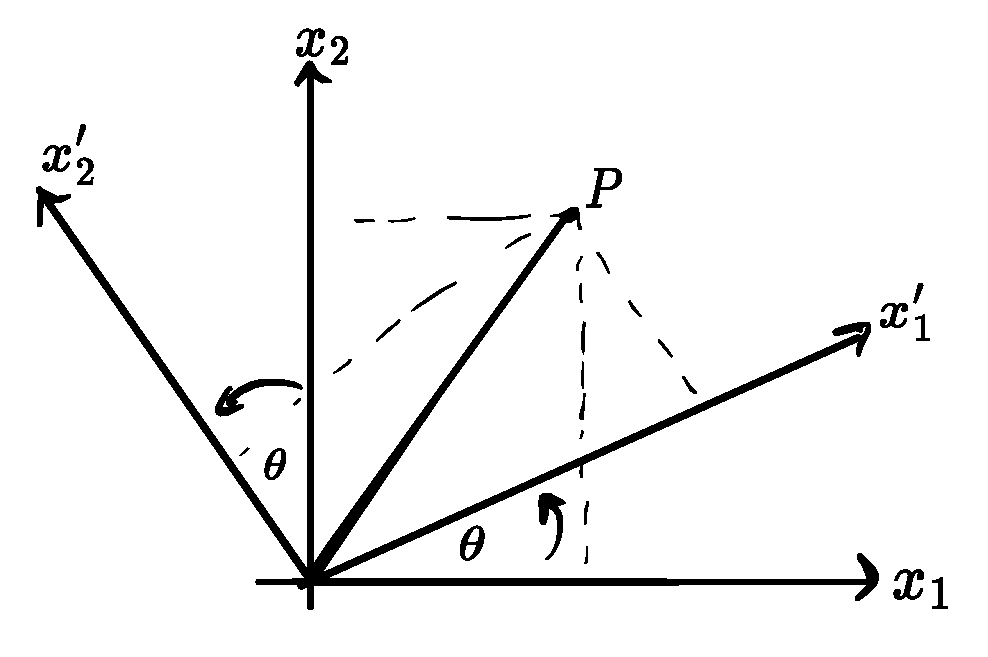
\includegraphics[scale=0.5]{sistema-coord.pdf}
%		\caption{Rotación en un plano.}
	\end{figure}
La relación entre las coordenadas primadas y las sin primar viene dada por
\begin{align}
  x'_1&=\cos\th x_1-\sin\th x_2\\
  x'_2&=\sin\th x_1+\cos\th x_2
\end{align}
o de manera equivalente
\begin{equation}
  \underbrace{\mqty(x_1'\\x'_2)}_{x'}=\underbrace{\mqty(\cos\th&-\sin\th\\\sin\th&\cos\th)}_{R(\th)}\underbrace{\mqty(x_1\\x_2)}_{x}
\end{equation}
Así, tenemos una transformación de la forma 
\begin{equation}
  x'=f(x,\th )
\end{equation}
además, notemos que 
\begin{itemize}
\item $\{R(\theta)\}$ tiene unidad $\forall \theta$, dada por
\begin{equation}
  R(0)=\mqty(1&0\\0&1)
\end{equation}
\item tiene inverso, $\forall\theta, \exists (-\theta)$.
\item es asociativo,
\item es conmutativo
\end{itemize}
Si la transformación $x'=f(x,\theta)$, entonces la unidad es dada por $x'=f(x,0)=f(x,e)=x$.
\end{ej}

\begin{defi}
	Un conjunto de transformaciones
	\begin{equation}
  x'^{i}=f^{i}(x',...,x^n;g^1,...,g^r)\equiv f(x,g)
\end{equation}
es llamado un \textbf{grupo de transformaciones $r$-paramétrico} si
\begin{enumerate}
	\item admite el elemento unidad
\begin{equation}
  x'=f(x,e)=x
\end{equation}
\item admite elemento inverso
\item tiene definida una ley de composición interna,
\begin{align}
  x'=f(x,g),\qquad x''=f(x',g')=f[f(x,g),g']=f(x,g'')
\end{align}
entonces 
\begin{equation}
  \boxed{g''=g''(g,g')}
\end{equation}
\end{enumerate}
\end{defi}
%
\begin{defi}
	Un conjunto de transformaciones es un \textbf{grupo de simetría} de una ecuación diferencial
	\begin{equation}\label{7.1}
  F(x,x^{(1)},...,x^{(n)})=0,\quad \text{con }x=(x^1,...,x^n)
\end{equation}
si la ecuación \eqref{7.1} permanece invariante en forma bajo la acción del grupo,
\begin{equation}
  F(x',x'^{(1)},...,x'^{(n)})=0
\end{equation}
\end{defi}

Lo interesante de los grupos de Lie es que basta estudiar sus versiones infinitesimales.
\begin{equation}
  x'=f(x,g)\to x'=f(x,\delta g)
\end{equation}
\begin{equation}
  x'^{i}=f^{i}(x,\delta g)=f^{i}(x,e)+\eval{\pdv{f^{i}(x,\delta g)}{g^k}}_{g=e}\delta g^k+\cdots
\end{equation}
donde $x'=f(x,e)=x$
\begin{equation}
  x'^{i}=x^{i}+\eval{\pdv{f^{i}(x,\delta g)}{g^k}}_{g=e}\delta g^k+\cdots
\end{equation}
\begin{equation}
  \Rightarrow \delta x^{i}=x'^{i}-x^{i}=\eval{\pdv{f^{i}(x,\delta g)}{g^k}}_{g=e}\delta g^k
\end{equation}
Esto significa que un cambio infinitesimal en los parámetros implica un cambio infinitesimal en las coordenadas de la variedad sobre la cual actúa el grupo.






















\newpage
\section{Clase 8}
\subsection{Generadores de grupos de Lie}
Sea $\M$ una variedad dotada de  sistemas de coordenadas $\{x_i\}_{i=1}^n$,$\{x'_i\}_{i=1}^n$ y sea $G$ un grupo $r$-paramétrico $a_\nu,\, \nu=1,...,r$. La acción del grupo $G$ sobre la variedad $\M$ es dada por el grupo de transformaciones 
\begin{equation}
  x'=f(x,a)  x'_i=f_i(x_j,a_\n )
\end{equation}
\begin{equation}
  x'_i=f_i(x_1,x_2,...,x_n; a_1,a_2,...,a_r)
\end{equation}
Para clarificar ideas consideremos el ejemplo de una variedad $\M$ de $2$ dimensiones que admite las coordenadas $x:(x_1,x_2)$ y $x':(x'_1,x'_2)$ y un grupo uni-paramétrico $G=SO(2)$ de rotaciones en el plano,

\begin{figure}[h!]
	\centering
	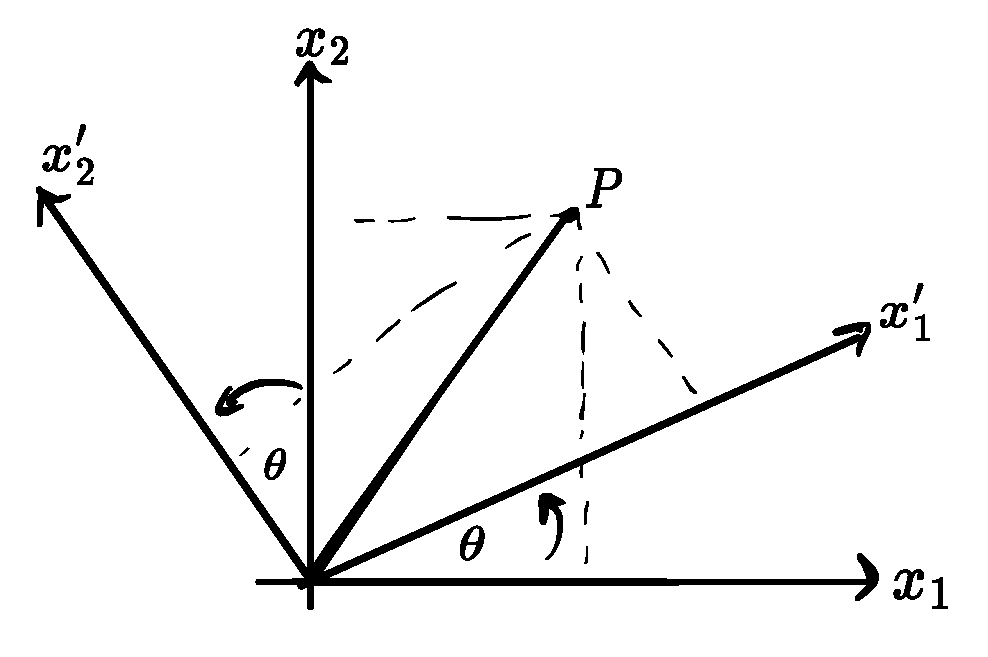
\includegraphics[scale=0.5]{sistema-coord.pdf}
\end{figure}

\begin{align}
  x'_1&=\cos\th x_1-\sin\th x_2\\
  x'_2&=\sin\th x_1+\cos\th x_2
\end{align}
o de manera equivalente
\begin{equation}
  \underbrace{\mqty(x_1'\\x'_2)}_{x'}=\underbrace{\mqty(\cos\th&-\sin\th\\\sin\th&\cos\th)}_{R(\th)}\underbrace{\mqty(x_1\\x_2)}_{x}
\end{equation}

\begin{equation}
  \implies x'=R(\th ) x \longleftrightarrow x'=f(x,\th )x
\end{equation}
o en general
\begin{equation}
  \implies x'=R(a ) x \longleftrightarrow x'=f(x,a )x
\end{equation}
De aquí vemos:
\begin{enumerate}
	\item La acción de $G=SO(2)$ es rotar las coordenadas de $\M$.
	\item Si el ángulo de rotación es pequeño, entonces el cambio experimentado por las coordenadas es también pequeño. Esto implica que en general, un pequeño cambio en los parámetros del grupo induce cambios pequeños en las coordenadas de $\M$.
\end{enumerate}

Notemos que cuando $\th =0$,
\begin{equation}
  R(0)=\mqty(1&0\\0&1)\implies \mqty(x'_1\\x'_2)=\mqty(1&0\\0&1)\mqty(x_1\\x_2)
\end{equation}
es decir,
\begin{equation}
  x'_1=x_1\quad x'_2=x_2
\end{equation}
\begin{equation}
  x'=R(0)x=x,\qquad  x'=f(x,0)=x
\end{equation}




Teniendo en cuenta que en el estudio de los grupos de Lie basta con estudiar su comportamiento infinitesimal, consideremos la expansión infinitesimal de la transformación $x'=f(x,a)$ alrededor de $a=0$.

\begin{equation}
  x'=f(x,a)=f(x,0)+\eval{\pdv{f(x,a)}{a}}_{a=0}\dd a+\cdots
\end{equation}
\begin{equation}
  x'_i=f_i(x_j,a_\n )=f_i(x_j,0)+\pdv{f_i(x_j,0)}{a_\nu }\dd a_\nu
\end{equation}
\begin{equation}
  x'=x+\pdv{f(x,a)}{a}\dd a
\end{equation}
\begin{equation}
  x'_i=x_i+\pdv{f_i(x,0)}{a_\nu}\dd a_\nu
\end{equation}
Esto implica que
\begin{equation}
  \dd x'=\pdv{f(x,0)}{a}\dd a,\qquad \dd x'_i=\pdv{f_i(x,0)}{a_\nu}\dd a_\nu
\end{equation}
Definiendo por comodidad
\begin{equation}
  u(x)=\pdv{f(x,0)}{a},\qquad u_{i\nu}(x)=\pdv{f_i(x,0)}{a_\nu}
\end{equation}
Así,
\begin{equation}\label{8.dxuda}
  \dd x=u(x)\dd a,\qquad \dd x_i=u_{i\nu}\dd a_\nu
\end{equation}
Notar que, de lo anterior\footnote{No estamos siendo estrictos con la posición de los índices coordenados de momento.}
\begin{equation}
 \boxed{ \dv{x_i}{a_\nu}=u_{i\nu}(x)}
\end{equation}
También podemos escribir
\begin{equation}
  \dd x_i=\sum _\n u_{i\nu }(x)\dd a_\n \qquad i=1,2,...,n,\qquad \n =1,2,...,r
\end{equation}

\begin{defi}
	Sea $F(x)=F(x_1,...,x_n)$ una función definida sobre la variedad $\M$. La función $F(x)$ es \textbf{invariante} bajo el grupo de transformaciones \begin{equation}
  x'=f(x,a)
\end{equation}
si $$F(x')=F[f(x,a)]=F(x).$$
\end{defi}

Consideremos ahora el cambio experimentado por la función $F(x)$ cuando cambian las coordenadas $x$ debido a un cambio en los parámetros del grupo.

Bajo un cambio en $x$ se tiene que $F(x)$ cambia como\footnote{El cambio en el parámetro genera un cambio en las coordenadas, y el cambio en las coordenadas genera un cambio en la función $F(x)$.}
\begin{align}
  \dd F&=\pdv{F}{x}\dd x=\pdv{F}{x}u(x)\dd a\\
  \dd F&=\dd a \l(u(x)\pdv{x}\r)F\\
  \dd F&=\dd a_\n \left(u_{i\n }(x)\pdv{x_i}\right)F
\end{align}
donde hemos usado \eqref{8.dxuda}.
\begin{defi}
	Se define el \textbf{generador} del grupo como el operador dado por
	\begin{equation}
  \boxed{X_\n =\sum_i u_{i\n }\pdv{x_i}},\qquad i=1,2,...,n,\qquad \n =1,2,...,r
\end{equation}
\end{defi}
Así, existe un generador por cada parámetro del grupo.

Esto implica que
\begin{equation}
  \dd F=\dd a_\n X_\n F\equiv XF
\end{equation}
donde
\begin{equation}
  X=\dd a_\n X_\n \equiv \dd a^\n X_\n 
\end{equation}

\begin{obs}
	Los generadores $X_\n$ son operadores que pueden o no ser operadores hermíticos. En el caso que ellos no sean hermíticos, pueden ser convertidos en hermíticos en general, multiplicándolos por $i$.
\end{obs}

\begin{teor}
	A partir de un conjunto de operadores hermíticos $X_\n$ podemos obtener una representación del grupo por medio de operadores unitarios
	\begin{equation}
 \boxed{U(a_\n )=e^{i a_\n X_\n }}
\end{equation}
\end{teor}

\begin{teor}
	Si $X_\n$ y $X_\m$ son generadores de un grupo de Lie, entonces
	su conmutador es una combinación lineal se dichos generadores:
	\begin{equation}
  [X_\n,X_\m ]=C_{\n\m}^{~~\lambda} X_\lambda \equiv C_{\m\n\lambda }X_\lambda
\end{equation}
donde
\begin{equation}
  C_{\n\m}^{~~\lambda}=-C_{\m\n }^{~~\lambda}
\end{equation}
\end{teor}
Dado que este producto es antisimétrico, satisface la \textbf{identidad de Jacobi},
\begin{equation}
  [[X_\m,X_\n ],X_\lambda]+[[X_\lambda,X_\m  ],X_\n ]+[[X_\n,X_\lambda ],X_\m ]=0
\end{equation}

\begin{ej}
	Consideremos el siguiente grupo de transformaciones 
	\begin{equation}\label{8.1}
  x'=\a_1x+\a_2,\qquad \a=(\a_1,\a_2)
\end{equation}
\begin{itemize}
	\item Encuentre los generadores del grupo
	\item Determine sus relaciones de conmutación
\end{itemize}
\end{ej}

\begin{sol}
	De \eqref{8.1} vemos que la identidad del grupo es dada por $\a_1=1$ y $\a_2=0$ ya que $x'=1x+0=x$, lo que implica que $\a_0=(\a_1^0,\a_2^0)=(1,0)$. Con el objeto de tener una identidad nula, definimos
	\begin{equation}
  a_1=\a_1-1,\qquad a_2=\a_2
\end{equation}
Es decir,
\begin{equation}
  a_1^0=\a_1^0-1,\qquad a_2^0=\a_2^0
\end{equation}
\begin{equation}
	\implies a_1^0=1-1=0,\qquad a_2^0=0
\end{equation}
\begin{equation}
  \implies a_0=(a_1^0,a_2^0)=(0,0)
\end{equation}
Así, el grupo de transformaciones toma la forma
\begin{equation}
  x'=(1+a_1)x+a_2
\end{equation}
\begin{equation}
  \implies\boxed{ x'=f(x,a)=x+a_1 x+a_2}
\end{equation}
\begin{equation}
  \implies \dd x_i=\pdv{f_i(x,0)}{a_\n }\dd a_\n =\uin \dd a_\n 
\end{equation}
\begin{equation}
  \dd x_i=\sum_\n \pdv{f_i}{a_\n }\dd a_\n 
\end{equation}
\begin{equation}
  \dd x_1\equiv \dd x=\pdv{f}{a_1}\dd a_1+\pdv{f}{a_2}\dd a_2
\end{equation}
\begin{equation}
  \dd x=x\dd a_1+1\dd a_2
\end{equation}
\begin{equation}
  \boxed{\dd x=x\dd a_1+\dd a_2}
\end{equation}
pero
\begin{equation}
  \dd x=u_{11}\dd a_1+u_{12}\dd a_2
\end{equation}
\begin{equation}
  \implies u_{11}=x,\qquad u_{12}=1
\end{equation}
de manera que 
\begin{equation}
  X_{\n }=\sum_i \uin \pdv{x_i}
\end{equation}
\begin{equation}
  X_1=u_{11}\pdv{x_1}=u_{11}\pdv{x}=x\pdv{x}
\end{equation}
\begin{equation}
  X_2=u_{12}\pdv{x_1}=u_{12}\pdv{x}=\pdv{x}
\end{equation}
Así, los generadores del grupo son
\begin{equation}
  X_1=x\pdv{x},\qquad X_2=\pdv{x}
\end{equation}
El conmutador es
\begin{align}
  [X_1,X_2]f&=X_1X_2f-X_2X_1f\\
  &=x\pdv{x}\left(\pdv{f}{x}\right)-\pdv{x}\left(x\pdv{f}{x}\right)\\
  &=x\pdv[2]{f}{x}-\pdv{f}{x}-x\pdv[2]{f}{x}\\
  &=-\pdv{f}{x}\\
  &=-X_2 f
\end{align}
\begin{equation}
  \implies [X_1,X_2]=-X_2
\end{equation}
Dado que
\begin{equation}
  [X_1,X_2]=C_{12}^{~~1}X_1+C_{12}^{~~2}X_2
\end{equation}
se tiene que las constantes de estructura son
\begin{equation}
  C_{12}^{~~1}=0,\qquad C_{12}^{~~2}=-1
\end{equation}
\end{sol}

\subsection{Grupos matriciales}
Sea $\M$ una variedad que admite las bases\footnote{Ver Ref. \cite{book:176834}} $\{\hat{e}_i\}_{i=1}^n$,$\{\hat{e}'_i\}_{i=1}^n$ y $\{\hat{e}''_i\}_{i=1}^n$ asociadas a las coordenadas $\{x_i\}_{i=1}^n$,$\{x'_i\}_{i=1}^n$ y $\{x''_i\}_{i=1}^n$. Un cambio de base es dado por
\begin{equation}
  \he'_j=B_j^{~i}\he_i,\qquad \he''_k=A_k^{~j}\he '_j,\qquad \he''_k=C_k^{~i}\he _i
\end{equation}
es decir,
\begin{equation}
  \he''_k=A_k^{~j}B_j^{~i}\he'_i=C_k^{~i}\he _i
\end{equation}
\begin{equation}
  \implies \boxed{C_k^{~i}=A_k^{~j}B_j^{~i}}
\end{equation}
Todas las bases de un espacio vectorial están relacionadas por medio de matrices. El conjunto de estas matrices constituyen un grupo.

\begin{defi}
	El conjunto de matrices $n\times n$ invertible que definen un cambio de base constituyen un grupo conocido como \textbf{grupo lineal general} definido sobre los espacios $\mathbb{R}^n,\mathbb{C}^n,\mathbb{Q}^n$. Estos grupos son denotados por $GL(n,\mathbb{R}),\, GL(n,\mathbb{C}),\, GL(n,\mathbb{Q})$.
\end{defi}

\subsubsection{Grupo general lineal $GL(n,\mathbb{C})$}
Grupo compuesto por todas las matrices complejas invertibles $n\times n$.

 Toda matriz $A\in GL(n,\mathbb{C}^n)$ tiene $2n^2$ elementos ($n^2$ elementos reales y $n^2$ elementos imaginarios).
 
 Este grupo tiene $2n^2$ parámetros reales, por lo cual tiene dimensión $2n^2$.
 
 \subsubsection{Grupo general lineal real $GL(n,\mathbb{R})$}
 Si exigimos que las matrices de $GL(n,\mathbb{C}^n)$ sean todas con elemento reales, obtenemos el grupo lineal general real $GL(n,\mathbb{R}^n)$, el cual tiene $n^2$ parámetros reales.
 
 \subsubsection{Grupo general lineal especial $SL(n,\mathbb{C})$}
 Si exigimos que todas las matrices de $GL(n,\mathbb{C})$ satisfagan las condiciones que tengan determinante $+1$, entonces obtenemos el grupo lineal especial $SL(n,\mathbb{C})$. Así, si $A\in SL(n,\mathbb{C})$, entonces $\det A=1$.
 
  \subsubsection{Grupo general lineal especial real $SL(n,\mathbb{R})$}
Si exigimos que todas las matrices de $GL(n,\mathbb{R})$ tengan determinante $+1$ entonces obtenemos el grupo especial lineal real $SL(n,\mathbb{R})$.










































\newpage
\section{Clase 9}
\subsubsection{Grupo unitario $U(n)$}
Es el grupo de todas las matrices complejas unitarias de $n\times n$. Esto significa que si $A\in U(n)$, entonces $A^\dagger A=1\implies A^\dagger=A$.

\subsubsection{Grupo especial unitario $SU(n)$}
Si exigimos a las matrices del grupo $U(n)$ que tengan determinante $1$, entonces obtenemos el grupo especial unitario $SU(n)$. Esto significa que si $A\in SU(n)$, entonces $A^\dagger A=1$ y $\det A=1$.

Ejemplos importantes en física son el grupo $SU(2)$ y el grupo $SU(3)$.

También son de gran importantes los grupos $SU(4)$, $SU(5)$ y $SU(6)$.

\underline{\textbf{Nota}}: El grupo $SU(2)\times U(1)$ está relacionado con las fuerzas electrodébiles (unificación del electromagnetismo con las fuerzas nucleares débiles). El grupo $SU(3)\times SU(2)\times U(1)$ está relacionado con la gran-unificación (unificación del electromagnetismo con las fuerzas nucleares débiles y fuertes).

\subsubsection{Grupo ortogonal $O(n,\mathbb{C})$}
Es el grupo de todas las matrices complejas ortogonales de $n\times n$. Esto significa que si $A\in O(n,\mathbb{C})$ entonces $A^TA=1\implies A^T=A^{-1}$.

\subsubsection{Grupo ortogonal especial $SO(n,\mathbb{C})$}
Si exigimos que las matrices del grupo $O(n,\mathbb{C})$ tengan determinante $1$, entonces obtenemos el grupo ortogonal especial $SO(n,\mathbb{C})$. Es decir, si $A\in SO(n)$\footnote{Por notación se puede omitir la $\mathbb{C}$.} entonces $A^TA=1$ y $\det A=1$

\subsection{Ejemplo: Generadores y álgebra de $SO(3)$}

\begin{ej}
	Determine los generadores del grupo ortogonal especial $3$-dimensional $SO(3)$ así como también su álgebra de Lie.
\end{ej}

\begin{sol}
	El grupo $SO(3)$ es el grupo de matrices ortogonales de $3\times 3$ y de determinante igual a $1$. La acción de $SO(3)$ sobre $E_3$ (o $\mathbb{R}^3$) es dada por el grupo de transformaciones 
	\begin{align}\label{9.1}
  x'=Ax
\end{align}
de aquí vemos que el elemento unidad es dado por $A_0=1\implies x'=A_0x=x$. Para lograr tener un elemento unidad nulo definimos 
\begin{align}
  a=A-1\implies a_0=A_0-1=1-1=0
\end{align}
así, la transformación \eqref{9.1} toma la forma
\begin{align}
  x'=f(x,a)=(1+a)x=x+ax
\end{align}
\begin{align}
  \dd x&=\dd a\pdv{f(x,0)}{a}\\
  &=\dd a x\label{9.2}
\end{align}
y recordamos que 
\begin{equation}\label{9.3}
  \dd x_i=\sum_\n u_{i\n }\dd a_\n 
\end{equation}
Dado que $A^TA=1$, tenemos que en el caso infinitesimal (a primer oden)
\begin{align} 
  (1+\dd a^T)(1+\dd a)&=1\\
  1+\dd a+\dd a^T+\cancel{\dd a^T\dd a}&=1
\end{align}
es decir, 
\begin{equation}
  \dd a=-\dd a^T
\end{equation}
explícitamente tenemos
\begin{equation}
  \mqty(\dd a_{11}&\dd a_{12}&\dd a_{13}\\
  \dd a_{21}&\dd a_{22}&\dd a_{23}\\
  \dd a_{31}&\dd a_{32}&\dd a_{33})=-\mqty(\dd a_{11}&\dd a_{21}&\dd a_{31}\\
  \dd a_{12}&\dd a_{22}&\dd a_{32}\\
  \dd a_{13}&\dd a_{23}&\dd a_{33})
\end{equation}
luego,
\begin{equation}
  \dd a=\mqty(0&\dd a_{12}&\dd a_{13}\\
  -\dd a_{12}&0&\dd a_{23}\\
  -\dd a_{13}&-\dd a_{23}&0)
\end{equation}
Definimos
\begin{equation}
  \dd a_{12}=\dd a_3,\qquad \dd a_{13}=-\dd a_2,\qquad \dd a_{23}=\dd a_1
\end{equation}
así
\begin{equation}
  \dd a=\mqty(0&\dd a_{3}&-\dd a_{2}\\
  -\dd a_{3}&0&\dd a_{1}\\
  \dd a_{2}&-\dd a_{1}&0)
\end{equation}
de \eqref{9.2}
\begin{align}
  \mqty(\dd x_1\\\dd x_2\\\dd x_3)=\mqty(0&\dd a_{3}&-\dd a_{2}\\
  -\dd a_{3}&0&\dd a_{1}\\
  \dd a_{2}&-\dd a_{1}&0) \mqty( x_1\\ x_2\\x_3)
\end{align}
obteniendo

\begin{equation}\label{9.4}
  \begin{split}
  \dd x_1&=x_2\dd a_3-x_3\dd a_2\\
  \dd x_2&=-x_1\dd a_3+x_3\dd a_1\\
  \dd x_3&=x_1\dd a_2-x_2\dd a_1
\end{split}
\end{equation}

De \eqref{9.3}
\begin{align}
  \dd x_1&=u_{11}\dd a_1+u_{12}\dd a_2+u_{13}\dd a_3\\
  \dd x_2&=u_{21}\dd a_1+u_{22}\dd a_2+u_{23}\dd a_3\\
  \dd x_3&=u_{31}\dd a_1+u_{32}\dd a_2+u_{33}\dd a_3
\end{align}
comparando
\begin{align}
  u_{11}&=0,\quad u_{12}=-x_3,\quad u_{13}=x_2\\
   u_{21}&=x_3,\quad u_{22}=0_3,\quad u_{23}=-x_1\\
    u_{31}&=-x_2,\quad u_{32}=x_1,\quad u_{33}=0
\end{align}
Los generadores vienen dados por
\begin{equation}
  X_\n =\sum_i \uin \pdv{x_i}
\end{equation}

\begin{align}
  X_1&=u_{11}\pdv{x_1}+u_{21}\pdv{x_2}+u_{31}\pdv{x_3}\\
  &=x_3\pdv{x_2}-x_2\pdv{x_3}\\
  X_2&=u_{12}\pdv{x_1}+u_{22}\pdv{x_2}+u_{32}\pdv{x_3}\\
  &=-x_3\pdv{x_1}+x_1\pdv{x_3}\\
  X_3&=u_{13}\pdv{x_1}+u_{23}\pdv{x_2}+u_{33}\pdv{x_3}\\
  &=x_2\pdv{x_1}-x_1\pdv{x_2}\\
\end{align}
en resumen,
\begin{tcolorbox}
\begin{align}
  X_1
  &=x_3\pdv{x_2}-x_2\pdv{x_3}\\
  X_2
  &=x_1\pdv{x_3}-x_3\pdv{x_1}\\
  X_3  &=x_2\pdv{x_1}-x_1\pdv{x_2}\\
\end{align}
\end{tcolorbox}

El conmutador
\begin{align*}
  [X_1,X_2]F&=X_1X_2F-X_2X_1F\\
  &=\left(x_3\pdv{x_2}-x_2\pdv{x_3}\right)\left(x_1\pdv{F}{x_3}-x_3\pdv{F}{x_1}\right)-\left(x_1\pdv{x_3}-x_3\pdv{x_1}\right)\left(x_3\pdv{F}{x_2}-x_2\pdv{F}{x_3}\right)\\
  &=x_3\pdv{x_2}\left(x_1\pdv{F}{x_3}\right)-x_3\pdv{x_2}\left(x_3\pdv{F}{x_1}\right)-
  x_2\pdv{x_3}\left(x_1\pdv{F}{x_3}\right)+x_2\pdv{x_3}\left(x_3\pdv{F}{x_1}\right)\\
  &-\left[x_1\pdv{x_3}\left(x_3\pdv{F}{x_2}\right)-x_1\pdv{x_3}\left(x_2\pdv{F}{x_3}\right)-x_3\pdv{x_1}\left(x_3\pdv{F}{x_2}\right)+x_3\pdv{x_1}\left(x_2\pdv{F}{x_3}\right)\right]\\
  &=\left(x_2\pdv{x_1}-x_1\pdv{x_2}\right)F\\
  &=X_3 F
\end{align*}
El cálculo para los demás conmutadores es análogo y se obtiene,
\begin{align}
  [X_1,X_2]&=X_3\\
  [X_3,X_1]&=X_2\\
  [X_2,X_3]&=X_1
\end{align}
o de manera compacta
\begin{equation}
  \boxed{[X_i,X_j]=\epsilon_{ijk}X_k}
\end{equation}
\end{sol}




























\newpage
\section{Clase 10}
\subsection{Generadores de transformaciones infinitesimales
}
Consideremos la siguiente transformación de simetría
\begin{align}
  q'^k&=q^k+\delta _\epsilon q^k=q^k+\epsilon\eta^k(q,t)\\
  t'&=t+\delta_\epsilon t=t+\epsilon\xi (t)
\end{align}

Tenemos transformaciones de simetría uni-paramétricas de parámetro $\epsilon$.

Para calcular los generadores, usamos el método usual
\begin{align}
  q'^k&=f^k(q^{i},\epsilon)=q^k+\epsilon \eta^k(q,t),\qquad\implies  \delta q^k=\epsilon\eta^k(q,t)\\
  t'&=f(t,\epsilon )=t+\epsilon\xi(t),\qquad \implies\delta t=\epsilon\xi(t)
\end{align}
Usaremos el siguiente esquema:
\begin{align}
  (q^k,\epsilon) &\Leftrightarrow x^{i}\implies x^1=q^k,\, x^2=t\\
  (f^k(q^{i},\epsilon),f(t,\epsilon))&\Leftrightarrow f^{i}(x^{i},a)
\end{align}
Recordemos que el generador viene dado por
\begin{equation}
  X_\n =\sum_{i}^2u_{i\n }\pdv{x_i},\qquad \n =1
\end{equation}
\begin{equation}
  X_1=u_{11}\pdv{x_1}+u_{21}\pdv{x_2}
\end{equation}
\begin{equation}
  u_{i\n }=\pdv{f^{i}}{a_\n }
\end{equation}
En este caso
\begin{align}
  u_{11}&=\pdv{f^k}{\epsilon}=\eta^k(q,t)\\
  u_{21}&=\pdv{f}{\epsilon}=\xi(t)
\end{align}
Así, el generador queda
\begin{equation}
  \boxed{X=\xi(q,t)\pdv{t}+\eta^k(q,t)\pdv{q^k}}
\end{equation}
Esto implica que
\begin{align}
  Xt&=\xi\pdv{t}{t}+\eta^k\pdv{t}{q^k}\\
  &=\xi 
\end{align}
\begin{align}
  Xq^k&=\xi\pdv{q^k}{t}+\eta^k\pdv{q^k}{q^k}\\
  &=\eta^k
\end{align}

Recordemos que una función $F(q,t)$ cambia bajo una transformación de simetría como
\begin{align}
  \d F=\epsilon XF=\epsilon\left(\xi\pdv{F}{t}+\eta^k\pdv{F}{q^k}\right)
\end{align}
Si la función $F(q,t)$ es generalizada al caso de una función $G(t,q,\qd,\ddot{q},...) $ el correspondiente generador se denota $\bar{X}$ tal que $\d G=\epsilon\bar{X}G$, donde 
\begin{align}
  X=\xi(t)\pdv{t}+\eta^k(q,t)\pdv{q^k}+\eta^k_{(1)}(t,q,\dot{q})\pdv{\qd^k}+\eta^k_{(2)}(t,q,\dot{q},\ddot{q})\pdv{\ddot{q}^k}+\cdots 
\end{align}


Hemos visto que
\begin{align}
  \d q^k&=\epsilon \eta^k\\
  \d t&=\epsilon\xi
\end{align}
Por otro lado sabemos
\begin{align}
  \db q^k&=\d q^k-\qd^k\d t\\
  &=\epsilon\eta^k-\qd^k\epsilon\xi\\
  &=\epsilon(\eta^k-\qd^k\xi)\equiv \epsilon \chi ^k
\end{align}
donde $\chi^k=\eta^k-\qd^k\xi$.

Recordemos que la corriente de Noether está dada por
\begin{align}
  J(t,q,\qd)&=\sum_i\pdv{L}{\qd_i}\db q_i+L\d t+\d\Omega\label{10.J}\\
  &=\sum_i\pdv{L}{\qd^{i}}\epsilon\chi^{i}+L\epsilon\xi+\epsilon\Omega\\
  &=\epsilon\left(\sum_i\pdv{L}{\qd^{i}}\chi^{i}+L\xi+\Omega\right)
\end{align}
Definimos la carga conservada como
\begin{align}
  J(t,q,\qd)&=\epsilon C(t,q,\qd)
\end{align}
donde
\begin{equation}
\boxed{  C(t,q,\qd)=\sum_i\pdv{L}{\qd^{i}}\chi^{i}+L\xi+\Omega}
\end{equation}
Esta carga es válida para transformaciones uni-paramétricas.

Consideremos ahora el caso de un grupo de transformaciones $r$-paramétricas de parámetro $\epsilon_\n $, $\n =1,2,...,r$,
\begin{align}
  \d_\epsilon q^k&=\epsilon^\n \eta^k_\n (t,q)\implies q'^k=f^k(q^k,\epsilon_\n )=q^k+\epsilon^\n \eta^k_\n \\
  \d_\epsilon t&=\epsilon^\n \xi_\n (t,q)\implies t'=f(t,\epsilon_\n )=t+\epsilon^n \xi_\n 
\end{align}
En este caso, los generadores son
\begin{align}
  X_{\n }=\sum_i^2 u_{i\n }\pdv{x_i},\qquad x_1\Leftrightarrow q^k,\, x_2\Leftrightarrow t
\end{align}
donde
\begin{align}
  u_{11}&=\pdv{f^k}{\epsilon_\n }=\eta^k_\n \\
  u_{21}&=\pdv{f}{\epsilon_\n }=\xi_\n 
\end{align}
Luego,
\begin{equation}
\boxed{  X_\n =\xi_\n \pdv{t}+\eta^k_\n \pdv{q^k}}
\end{equation}
Estos generadores tienen la propiedad que el producto antisimétrico de dos de ellos da lugar a un tercer generador, de acuerdo a
\begin{equation}
 \boxed{ [X_\m ,X_\n ]=\Upsilon_{\m\n\lambda}X_\lambda}
\end{equation}
En el caso que $\Upsilon_{\m\n\lambda}$ sea constante, este producto genera un \textit{álgebra de Lie}.

\subsection{Cargas conservadas}
La corriente conservada es dada por \eqref{10.J} 
\begin{equation}
   J(t,q,\qd)=\sum_i\pdv{L}{\qd_i}\db q_i+L\d t+\d\Omega
\end{equation}
donde
\begin{align}
  \d t&=\epsilon^\n \xi_n\\
  \d q^k&=\epsilon^\n \eta^k_\n 
\end{align}
de donde se desprende
\begin{align}
  \db q^{i}&=\d q^{i}-\qd^{i}\d t\\
  &=\epsilon^\n \eta^{i}_\n -\qd^{i}\epsilon^\n \xi_\n \\
  &=\epsilon^\n (\eta^{i}_\n -\qd^{i} \xi_\n )\\
  &=\epsilon^\n \chi ^k_\n 
\end{align}
donde $\chi^k_\n =\eta^{i}_\n -\qd^{i} \xi_\n $. Así,
\begin{align}
  J(t,q,\qd)&=\sum_i\pdv{L}{\qd_i}\epsilon^\n \chi^{i}_\n +L\epsilon^\n \xi_\n +\epsilon^\n \Omega_\n \\
  &=\epsilon^\n \left(\sum_i\pdv{L}{\qd_i} \chi^{i}_\n +L \xi_\n +\Omega_\n \right)\\
  &\equiv \epsilon^\n C_\n 
\end{align}
donde
\begin{equation}
  C_\n =\sum_i\pdv{L}{\qd_i} \chi^{i}_\n +L \xi_\n +\Omega_\n 
\end{equation}
es la llamada \textbf{carga conservada de Noether}.

Dado que
\begin{equation}
  \chi^k_\n =\eta^{i}_\n -\qd^{i} \xi_\n 
\end{equation}
tenemos
\begin{align}
  C_\n &=\sum_i\pdv{L}{\qd_i} (\eta^{i}_\n -\qd^{i} \xi_\n ) +L \xi_\n +\Omega_\n \\
  &=\sum_i\pdv{L}{\qd^{i}}\eta^{i}_\n -\sum_i\left(\pdv{L}{\qd^{i}}\qd^{i}-L\right)\xi_\n +\Omega_\n \\
  &=\sum_i\pdv{L}{\qd^{i}}\eta^{i}_\n -\sum_i\left(p_i\qd^{i}-L\right)\xi_\n +\Omega_\n 
\end{align}
\begin{equation}
  \implies \boxed{C_\n =\sum_i\pdv{L}{\qd^{i}}\eta^{i}_\n -H_c\xi_\n +\Omega_\n }
\end{equation}
donde $H_c$ corresponde al \textit{Hamiltoniano canónico}.

\begin{teor}
	La variación de las coordenadas es dada en función de las cargas de Noether por medio de 
	\begin{equation}
  \db q^k=[q^k,\epsilon^\n C_\n ]
\end{equation}
donde $[,]$ es el corchete de Poisson.
\end{teor}

\begin{prueba}
	Calculemos
	\begin{align}
  [q^k,\epsilon^\n C_\n ]&=\left[q^k,\epsilon^\n \left(\sum_i\pdv{L}{\qd^{i}}\eta^{i}_\n -H_c\xi_\n +\Omega_\n \right)\right]\\
  &=\left[q^k,\epsilon^\n \sum_ip_i\eta^{i}_\n \right]-\left[q^k,\epsilon ^\n H_c\xi_\n \right]+\cancelto{0}{[q^k,\epsilon^\n \Omega_\n ]},\qquad \Omega_\n =\Omega_\n (q,t)\\
  &=\sum_i\epsilon^\n [q^k,p_i]\eta^{i}_\n -\epsilon^\n [q^k,H_c]\xi_\n \\
  &=\sum_i\epsilon^\n \delta^k_i\eta^{i}_\n -\epsilon^\n \qd^k\xi_\n \\
  &=\epsilon^\n \eta^k_\n -\epsilon^\n \qd^k\xi_\n \\
  &=\epsilon^\n( \eta^k_\n - \qd^k\xi_\n )\\
  &=\epsilon^\n \chi^k_\n \\
  &=\db q^k
\end{align}
Así,
\begin{equation}
  \db q^k=[q^k,\epsilon^\n C_\n ]\qquad \qed
\end{equation}
\end{prueba}


\begin{teor}
	Las cargas de Noether satisfacen la siguiente relación de conmutación
	\begin{equation}\label{10.0}
  [C_\m,C_\n]=\Upsilon_{\m\n\lambda}C_\lambda + Z_{\m\n }
\end{equation}
\end{teor}

\begin{prueba}
	Hemos visto que $\db q^k=[q^k,\epsilon^\n C_\n ]$. Consideremos el conmutador de dos transformaciones $\db$,
	\begin{align}
  \db_1 q^k&=[q^k,\epsilon_1^\n C_\n ]\\
  \db_2(\db_1 q^k)&=[\db_1q^k,\epsilon^\m_2C_\n ]=[[q^k,\epsilon_1^\n C_\n ],\epsilon_2^\m C_\m ]\\
  \implies \db_2\db_1 q^k&=\epsilon_1^\n \epsilon_2^\n [[q^k,C_\n ],C_\m ]\label{10.1}
\end{align}
Además,
\begin{align}
  \db_1(\db_2  q^k)&=[\db_2 q^k,\epsilon^\m _1C_\m ]=[[q^k,\epsilon_2^\n C_\n ]\epsilon_1^\m ,C_\m ]\\
  &=\epsilon_2^\n \epsilon_1^\m [[q^k,C_\n ],C_\m ]
\end{align}
Así,
\begin{align}
  \db_2\db_1q^k-\db_1\db_21^k&=\epsilon_1^\n \epsilon_2^\m [[q^k,C_\n ],C_\m] -\epsilon_2^\n \epsilon_1^\n [[q^k,C_\n],C_\m ]\\
  &=\epsilon_1^\m \epsilon_2^\n \left\{[[q^k,C_\m ],C_\n ]-[[q^k,C_\n ],C_\m ]\right\}
\end{align}
De la identidad de Jacobi,
\begin{equation}
  [[q^k,C_\m ],C_\n ]+ [[C_\n ,q^k ],C_\m  ]+ [[C_\m ,C_\n  ],q^k ]=0
\end{equation}
lo que implica que
\begin{equation}\label{10.3}
  \db_2\db_1q^k-\db_1\db_2q^k=\epsilon_1^\m \epsilon_2^\n [q^k,[C_\m,C_\n ]]
\end{equation}
Dado que el producto de dos transformaciones debe dar lugar a una tercera transformación
\begin{equation}
  [\db_2,\db_1]q^k=\db_3q^k=[q^k,\epsilon^\lambda C_\lambda]
\end{equation}
luego, podemos conjeturar que $\epsilon^\lambda\sim \epsilon_1^\m \epsilon_2^\n $, de manera que $[C_\m ,C_\n ]\sim C_\lambda$. Para hacer consistente la conjetura introducimos \eqref{10.0} en \eqref{10.3}
\begin{align}
  \epsilon_1^\m \epsilon_2^\n [q^k,[C_\m,C_\n ]]&=\epsilon_1^\m \epsilon_2^\n[q^k, \Upsilon_{\m\n\lambda}C_\lambda+Z_{\m\n }]\\
  &=\Upsilon_{\m\n\lambda}\epsilon_1^\m \epsilon_2^\n[q^k,C_\lambda]+\epsilon_1^\m \epsilon_2^\n\cancelto{0}{[q^k,Z_{\m\n }]},\qquad \text{($q$ conmuta con $Z$)}
\end{align}
\begin{equation}
  [\db_2,\db_1]q^k=\Upsilon_{\m\n\lambda}\epsilon_1^\m \epsilon_2^\n[q^k,C_\lambda]=\epsilon^\lambda[q^k,C_\lambda]
\end{equation}
\begin{equation}
  \implies \epsilon^\lambda=\Upsilon_{\m\n\lambda }\epsilon_1^\m \epsilon_2^\n
\end{equation}1
\end{prueba}




























































\newpage
\section{Clase 11}
\subsection{Grupo de Galileo y sus cargas conservadas}
Consideremos la función de Lagrange 
\begin{equation}
  L=\frac{1}{2}\sum_i m_i\dot{x}^2_i+\sum_{i<j}V|x_i-x_j|
\end{equation}
es invariante bajo el grupo de Galileo. A saber,

\textbf{Traslaciones temporales:} $G_\t :t'=t+\t =f(t,\t )$. 

Siguiendo el procedimiento usual, $a_\n \leftrightarrow \t ,\, \n =1$ y $x_i\leftrightarrow t$. Luego
\begin{equation}
  u_{11}=1,\quad X_\n =\sum_i u_{i\n }\pdv{x_i}
\end{equation}
\begin{equation}
  X=\pdv{t}=H\implies H=\pdv{t}
\end{equation}

\textbf{Traslaciones espaciales:} $G_a :x'=x_i+a_i=f(x_{i},a_{i})$.
\begin{equation}
  u_{11}=1,\qquad X=\pdv{x_i}\implies P_i=\pdv{x}
\end{equation}

\textbf{Rotaciones temporales:} $G_R :x'=x_i+R_{i}^j x_j=f(x_{i},\th )$.

Anteriormente determinamos los generadores de $SO(3)$,
\begin{align}
  X_{12}&=x_1\pdv{x_2}-x_2\pdv{x_1} \quad \longrightarrow X_3\\
  X_{23}&=x_2\pdv{x_3}-x_3\pdv{x_2}\quad \longrightarrow X_1\\
  X_{31}&=x_3\pdv{x_1}-x_1\pdv{x_3}\quad \longrightarrow X_2
\end{align}
de manera que
\begin{equation}
  X_i=\epsilon_{ijk}x_j\pdv{x^k}\equiv J_i
\end{equation}

\textbf{Boosts de Galileo:} $G_v :x'=x_i+v_it=f(x_i,v_i)$.
\begin{equation}
  u_{11}=t,\qquad X_i=t\pdv{x^{i}},\qquad G_i=t\pdv{x^{i}}\equiv t P_i
\end{equation}

Así tenemos que los generadores del grupo de Galileo son $\{H,P_i,J_i,G_i\}$ donde
\begin{align}
  H&=\pdv{t}\\
  P_i&=\pdv{x^{i}}\\
  J_i&=\epsilon_{ijk}x_j\pdv{x^k}\\
  G_i&=t\pdv{x^{i}}
\end{align}

\subsection{Partícula libre en $3$-dimensiones}
Las ecuaciones de Newton son invariantes bajo el grupo de transformaciones de Galileo. Normalmente es aceptado que las transformaciones de Galileo son las simetrías más generales bajo la cual las ecuaciones de Newton permanecen invariantes en forma.

Sin embargo, notemos que la trayectoria de una partícula libre que parte desde $\vec{x}_0$ con velocidad $\vec{v}_0$ es igual a 
\begin{equation}\label{11.1}
  \vec{x}(t)=\vec{x}_0+\vec{v}_0t
\end{equation}
que relaciona las posiciones de la partícula. Escribiendo \eqref{11.1} en la forma
\begin{equation}\label{11.2}
  \frac{\vec{x}(t)}{t}=\frac{\vec{x}_0}{t}+\vec{v}_0
\end{equation}
Si llamamos $\tilde{\vec{x}}(t)=\vec{x}(t)/t$ y $\tilde{t}=1/t$, tenemos
\begin{equation}
  \tilde{\vec{x}}(t)=\vec{v}_0+\vec{x}_0\tilde{t}
\end{equation}
que relaciona velocidades. Notemos que existe una dualidad entre \eqref{11.1} y \eqref{11.2}.

En Ref. \cite{Jahn:2001qk} fue encontrado que el grupo de transformaciones más general que deja invariante la ecuación de Newton es un grupo de $12$ generadores ($12$ parámetros) constituido por
\begin{itemize}
	\item El grupo de Galileo de $10$ parámetros.
	\item El grupo de dilataciones de $1$ parámetro.
	\item El grupo de expansiones de $1$ parámetro.
\end{itemize}

 Los generadores de este grupo general son:
\begin{align*}
  H&=\pdv{t}\\
  P_i&=\pdv{q^{i}}\\
  J_i&=\epsilon_{ijk}q_j\pdv{q^k}\\
  G_i&=t\pdv{q^{i}}\\
  S&=2t\pdv{t}+q^{i}\pdv{q^{i}}\\
  C&=t^2\pdv{t}+tq^{i}\pdv{q^{i}}
\end{align*}
Este grupo es conocido como el \textit{grupo de Schrödinger} que también deja invariante la ecuación de Schrödinger (Ver Ref. \cite{Niederer:1972zz}).

\part{Electrodinámica y Relatividad}
\subsection{Transformaciones de Galileo y ecuaciones de Newton}
Consideremos dos SRI $K$ y $K'$. La relación entre las mediciones de ambos SRI está dado por
\begin{equation}
  x'=x-vt,\qquad y'=y,\qquad z'=z,\qquad t'=t
\end{equation}

\begin{figure}[h!]
	\centering
	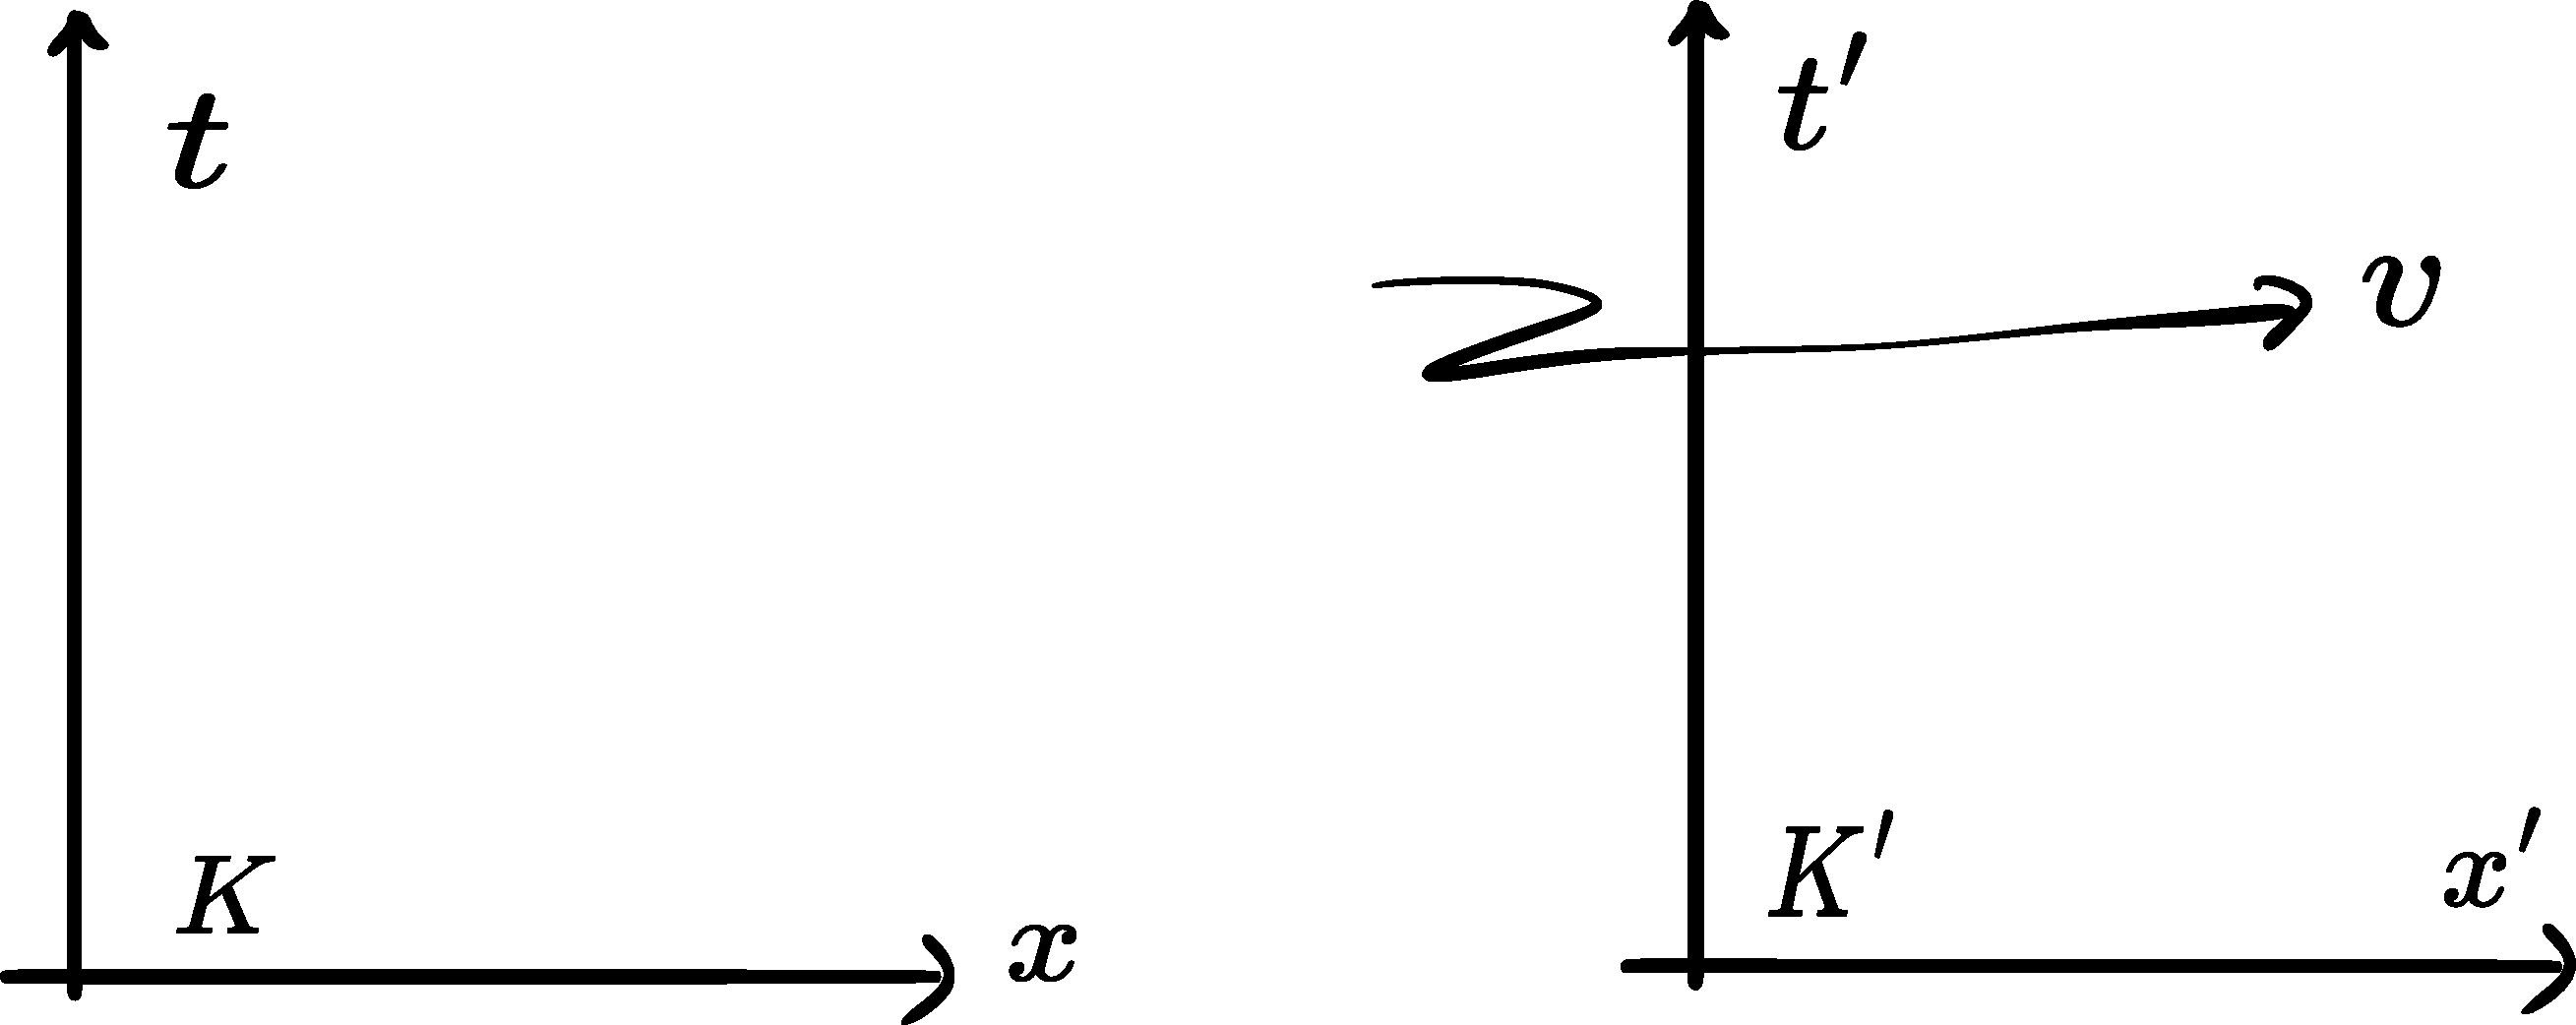
\includegraphics[scale=0.2]{fig/Galileo.pdf}
\end{figure}

La covariancia de las leyes de la física implican que las leyes de Newton en $K$ deben tener la misma forma en $K'$,
\begin{align}
  K&:\quad \vec{F}=m\vec{a}\\
  K'&:\quad \vec{F}'=m'\vec{a}'
\end{align}
Veamos si $F=ma$ es invariante bajo Galileo: \footnote{Por simplicidad consideremos una sóla dimensión.}
\begin{equation}
  x'=x-vt\implies \dv{x'}{t'}=\dv{x}{t}-v
\end{equation}
Definiendo la velocidad medida en $K$ con $V=\dv*{x}{t}$ y la velocidad medida en $K'$ con $V'=\dv*{x'}{t'}$ tenemos
\begin{equation}
  V'=V-v\implies \boxed{V'\neq V}
\end{equation}
es decir, la velocidad es una cantidad relativa.

\begin{equation}
  \dv{V'}{t'}=\dv{V}{t}-\dv{v}{t}
\end{equation}
pero $v$ es constante, luego
\begin{equation}
  \dv{V'}{t'}=\dv{V}{t}\implies \boxed{a'=a}
\end{equation}
es decir, la aceleración es una cantidad absoluta. Dado que por postulado la masa es una cantidad absoluta $m'=m$, se tiene
\begin{equation}
\boxed{  F'=F}
\end{equation}

 En este punto es natural hacerse la siguiente pregunta: ¿Son todas las leyes de la física invariante en forma? o ¿Son todas las leyes de la física invariantes en forma bajo Galileo?
 
 Las ecuaciones de Maxwell en el vacío vienen dadas por:
 \begin{align}
  &\nabla\cdot\vec{E}=0\label{11.11}\\
  &\nabla\cdot\vec{B}=0\label{11.12}\\
  &\nabla\times \vec{E}=-\pdv{\vec{B}}{t}\label{11.13}\\
  &\nabla\times \vec{B}=\m_0\ep_0\pdv{\vec{E}}{t}\label{11.14}
\end{align}
tomando el rotacional de \eqref{11.13} tenemos
\begin{align}
  \nabla\times \nabla \times\vec{E}&=-\nabla\times \pdv{\vec{B}}{t}=-\pdv{t}(\nabla\times\vec{B})\\
  &=-\pdv{t}\left(\m_0\ep_0\pdv{\vec{E}}{t}\right)\\
  &=-\m_0\ep_0\pdv[2]{\vec{E}}{t}
\end{align}
usando la identidad del cálculo vectorial, se tiene
\begin{align}
  \nabla(\cancelto{0}{\nabla\cdot\vec{E}})-\nabla^2\vec{E}=-\m_0\ep_0\pdv[2]{\vec{E}}{t}
\end{align}
\begin{equation}
  \implies \nabla^2\vec{E}-\m_0\ep_0\pdv[2]{\vec{E}}{t}=0
\end{equation}
Del mismo modo tenemos
\begin{equation}
  \nabla^2\vec{B}-\m_0\ep_0\pdv[2]{\vec{B}}{t}=0
\end{equation}
Cada componente $E_x,E_y,E_z,B_x,B_y,B_z$ satisface la ecuación
\begin{equation}\label{11.onda}
  \nabla^2\psi-\frac{1}{c^2}\pdv[2]{\psi}{t}=0,\qquad c^2=\frac{1}{\m_0\ep_0}
\end{equation}



\begin{ej}
	Probar que las ecuaciones de Maxwell no son invariantes bajo las transformaciones de Galileo, es decir, que las ecuaciones de Maxwell cambian de forma.
\end{ej}
\begin{sol}
	\begin{equation}
  x'=x-vt,\qquad y'=y,\qquad z'=z,\qquad t'=t
\end{equation}
esto implica que
\begin{equation}
  \pdv{x'}{x}=1,\qquad \pdv{x'}{t}=-v,\qquad \pdv{t'}{x}=0,\qquad \pdv{t'}{t}=1
\end{equation}
Luego,
\begin{equation}\label{11.trans}
\begin{split}
  \pdv{x}&=\pdv{x'}\pdv{x'}{x}+\pdv{t'}\pdv{t'}{x}=\pdv{x'}\\
  \pdv{t}&=\pdv{x'}\pdv{x'}{t}+\pdv{t'}\pdv{t'}{t}=\pdv{t'}-v\pdv{x'}
 \end{split}
\end{equation}
Las ecuaciones de Maxwell en una dimensión quedan
\begin{align}
  \nabla\cdot\vec{E}=0&\Longrightarrow \pdv{E_x}{x}=0\\
  \nabla\cdot\vec{B}=0&\Longrightarrow \pdv{B_x}{x}=0\\
  \nabla\times \vec{E}=-\pdv{\vec{B}}{t}&\Longrightarrow \pdv{E_z}{y}-\pdv{E_y}{z}=-\pdv{B_x}{t}\\
  \nabla\times \vec{B}=\m_0\ep_0\pdv{\vec{E}}{t}&\Longrightarrow \pdv{B_z}{y}-\pdv{B_y}{z}=\m_0\ep_0\pdv{E_x}{t}\\
\end{align}
Aplicando la transformación de Galileo, de \eqref{11.trans} se tiene
\begin{align}
  \pdv{E_x'}{x'}&=0\\
  \pdv{B_x'}{x'}&=0\\
  \pdv{E_z'}{y'}-\pdv{E_y'}{z'}&=-\pdv{B_x'}{t'}=-\left(\pdv{B_x'}{t'}-v\pdv{B_x'}{x'}\right)\\
  \pdv{B_z'}{y'}-\pdv{B_y'}{z'}&=\m_0\ep_0\pdv{E_x'}{t'}=\m_0\ep_0\left(\pdv{E_x'}{t'}-v\pdv{E_x'}{x'}\right)
\end{align}
Notar que estas dos últimas ecuaciones cambian en forma. Luego, bajo transformaciones de Galileo las ecuaciones de Maxwell cambian en forma.
\end{sol}

\begin{ej}
	Probar que la ecuación de la onda \eqref{11.onda} no es invariante bajo transformaciones de Galileo.
\end{ej}

























































\newpage
\section{Clase 12}
Hemos visto que las ecuaciones d Newton son invariantes en forma bajo las transformaciones de Galileo. Dado que las estas transformaciones sólo son validas en SRI, los cuales están relacionados por transformaciones de Galileo, se tiene que por medio de elemento mecánicos no es posible determinar si un sistema está en reposo o MRU ya que todos los SRI son equivalentes a los ojos de las transformaciones de Galileo.

Las ecuaciones de Maxwell \textit{no son invariantes} bajo transformaciones de Galileo, lo cual implica que no todos los SRI son equivalentes a los ojos de las ecuaciones de Maxwell. Es decir, existen sistemas de referencia privilegiados para las ecuaciones de Maxwell. Dichas ecuaciones adquieren si forma más simple en el SRI donde fueron escritas por Maxwell. Este SRI es privilegiado con respecto a los SRI que se mueven con respecto al sistema de referencia de Maxwell. Al SRI de Maxwell se le postula como en reposo con respecto al éter.

Por medio de experimentos electromagnéticos (por ejemplo, óptico) podría ser posible determinar si un SRI está en reposo ó en MUR con respecto del sistema del éter.

En este contexto se llevó a cabo el experimento de Michelson-Morley. El resultado de dicho experimento no encontró evidencia del éter ni como saber si un cuerpo estaba en reposo o en MUR.

 Esto implicó que las ecuaciones de Maxwell deberían ser invariantes bajo un grupo de transformaciones. Lorentz encontró un grupo de transformaciones que dejaba invariante las ecuaciones de Maxwell. Dichas transformaciones sólo eran válidas para la electrodinámica.
 
 Einstein postuló que debían existir transformaciones válidas para toda la física y estableció el principio de covariancia general: \textit{toda la física debe ser invariante en forma bajo un conjunto de transformaciones}. Estas transformaciones deberían ser obtenidas a partir de principios fundamentales del espacio y del tiempo.
 
 Einstein postuló que dichos principio eran:
 \begin{enumerate}
 	\item[i)] \textbf{Homogeneidad del tiempo}: todos los instantes son equivalentes.
 	\item[ii)] \textbf{Homogeneidad e isotropía del espacio}: todos los puntos y las direcciones son equivalentes.
 	\item[iii)] \textbf{Principio de la relatividad}: todos los SRI son equivalentes para \textit{toda} la física. (No sólo para la mecánica).
 	\item[iv)] \textbf{Postulado de la constancia de la velocidad de la luz}.
 \end{enumerate}
 
 A partir de estos principios Einstein encontró que las transformaciones buscadas eran las transformaciones de Lorentz:
 \begin{align}
 t'&=\frac{\left(t-\dfrac{v}{c^2}x\right)}{\sqrt{1-v^2/c^2}}\\
  x'&=\frac{(x-vt)}{\sqrt{1-v^2/c^2}}\\
y'&=y\\
z'&=z
\end{align}
llamaremos $\g=\frac{1}{\sqrt{1-v^2/c^2}}$ y $x^0=ct$. Escribiendo estas transformaciones como
\begin{align}
x'^0&=\g\left(x^0-\frac{v}{c}x^1\right)\\
  x'^1&=\g\left(x^1-\frac{v}{c}x^0\right)\\
  x'^2&=x^2\\
  x'^3&=x^3
\end{align}
o de manera equivalente
\begin{align}
  x'^0&=\g x^0-\g \frac{v}{c}x^1\\
  x'^1&=-\g \frac{v}{c}x^0+\g x^1\\
  x'^2&=x^2\\
  x'^3&=x^3
\end{align}
Escribiendo estas transformaciones en forma matricial, se tiene
\begin{equation}
  \underbrace{\mqty(x'^0\\x'^1\\x'^2\\x'^3)}_{x'^\m }=\underbrace{\mqty(\g&-\g\frac{v}{c}&0&0\\
  -\g\frac{v}{c}&\g&0&0\\
  0&0&1&0\\0&0&0&1)}_{\Lambda^\m _{~\n }}\underbrace{\mqty(x^0\\x^1\\x^2\\x^3)}_{x^\n }
\end{equation}
\begin{equation}
  \implies \boxed{x'^\m =\Lambda^\m_{~\n }x^\n }
\end{equation}
donde en general
\begin{equation}
  \Lambda^\m_{~\n }=\mqty(\Lambda^0_{~0}&\Lambda^0_{~1}&\Lambda^0_{~2}&\Lambda^0_{~3}\\\Lambda^1_{~0}&\Lambda^1_{~1}&\Lambda^1_{~2}&\Lambda^1_{~3}\\\Lambda^2_{~0}&\Lambda^2_{~1}&\Lambda^2_{~2}&\Lambda^2_{~3}\\\Lambda^3_{~0}&\Lambda^3_{~1}&\Lambda^3_{~2}&\Lambda^3_{~3})
\end{equation}

De la Relatividad Especial, sabemos que el principio de constancia de la velocidad de la luz implica que la distancia entre dos puntos del espacio de Minkowski es invariante bajo transformaciones de Lorentz,
\begin{align}
  S^2&=x^\m x_\m =\eta_{\m\n }x^\m x^\n \\
  S'^2&=x'^\m x'_\m =\eta_{\m\n }x'^\m x'^\n 
\end{align}
La invariancia de $S^2$ nos dice
\begin{equation}
  S'^2=S^2
\end{equation}
\begin{equation}
  \implies \eta_{\m\n }x'^\m x'^\n =\eta_{\m\n }x^\m x^\n
\end{equation}
pero
\begin{equation}
  x'^\m =\Lambda^\m_{~\n }x^\n 
\end{equation}
luego,
\begin{equation}
  \implies \eta_{\m\n }\Lambda^\m_{~\a}x^\alpha \Lambda^\n _{~\b }x^\b =\eta_{\a\b  }x^\a  x^\b 
\end{equation}
\begin{equation}
  \implies \eta_{\m\n }\Lambda^\m_{~\a} \Lambda^\n _{~\b }x^\a x^\b =\eta_{\a\b  }x^\a  x^\b 
\end{equation}
\begin{equation}
  \implies\boxed{ \eta_{\m\n }\Lambda^\m_{~\a} \Lambda^\n _{~\b }=\eta_{\a\b  }}
\end{equation}
o en forma matricial
\begin{equation}
\boxed{  \Lambda^T\eta\Lambda=\eta}
\end{equation}

\begin{teor}
	Las matrices $\Lambda^\m_{~\n }$ constituyen un grupo de Lie no-compacto conocido como \textit{grupo de Lorentz} definido como
	\begin{equation}
  L:=O(1,3)=\{\Lambda\in GL(4,\mathbb{R})/\Lambda^T\eta\Lambda=\eta\}
\end{equation}
el cual tiene asociada un álgebra de Le conocida como el \textit{álgebra de Lorentz}, definida como
\begin{equation}
  \mathfrak{o}(1,3)=\{a\in M_{4\times 4}(\mathbb{R})/a^T=-\eta a\eta\}
\end{equation}
\end{teor}

\begin{prueba}
	De la teoría de las álgebras de Lie sabemos que un elemento de un grupo y un elemento del álgebra están relacionados por exponenciación, a saber
	\begin{equation}
  \Lambda=e^{ta},\quad \Lambda\in O(1,3),\quad a\in \mathfrak{o}(1,3)
\end{equation}
donde $t$ son los parámetros del grupo.

Las matrices $\Lambda$ satisfacen la condición
\begin{equation}
  \Lambda^T\eta\Lambda=\eta
\end{equation}
\begin{equation}
  \implies [e^{ta}]^T\eta [e^{ta}]=\eta 
\end{equation}
para determinar las condiciones del álgebra debemos remitirnos a la vecindad de la identidad de las $\Lambda$,
\begin{equation}
  \Lambda =e^{ta}\implies \Lambda=1\text{ ocurre en } t=0
\end{equation}
\begin{align}
  \implies \dv{t}\eval{\left([e^{ta}]^T\eta [e^{ta}]\right)}_{t=0}&=\dv{t}\eval{\eta}_{t=0}\\
  \dv{t}\eval{[e^{ta}]^T\eta [e^{ta}]}_{t=0}+\eval{[e^{ta}]^T\eta \dv{t}[e^{ta}]}_{t=0}&=0\\
  \eval{[ae^{ta}]^T\eta [e^{ta}]}_{t=0}+\eval{[e^{ta}]^T\eta [ae^{ta}]}_{t=0}&=0\\
  [a]^T\eta +\eta [a]&=0\\
  a^T\eta +\eta a&=0
\end{align}
multiplicando por $(\cdot \eta^{-1}\equiv\eta )$, se tiene
\begin{align}
  a^T+\eta a\eta=0
\end{align}
\begin{equation}
  \implies \boxed{a^T=-\eta a\eta} \qed 
\end{equation}
\end{prueba}

\begin{teor}
	Los constraints
	\begin{equation}
  \det\Lambda=\pm 1\quad \text{y}\quad |\Lambda^0_{~0}|\geq 1
\end{equation}
definen $4$ partes desconectadas en el espacio de los parámetros del grupo de Lorentz.
\end{teor}

\begin{prueba}
	Sabemos que las matrices de Lorentz satisfacen la condición
	\begin{equation}
  \Lambda^T\eta \Lambda=\eta
\end{equation}
\begin{align}
  \implies \det (\Lambda^T\eta)&=\det\eta \\
  (\det\Lambda^T)\underbrace{(\det\eta)}_{-1}(\det\Lambda)&=\underbrace{\det\eta}_{-1} \\
  (\det\Lambda)^2&=1
\end{align}
\begin{equation}
  \implies \boxed{\det\Lambda=\pm 1}
\end{equation}
Por otro lado, dado que
\begin{equation}
  \eta_{\a\b }=\eta_{\m\n}\Lambda^\m_{~\alpha}\Lambda^\n_{~\b }
\end{equation}
\begin{equation}
  \implies \eta_{00 }=\eta_{\m\n}\Lambda^\m_{~0}\Lambda^\n_{~0 }=\eta_{00}\Lambda^0_{~0}\Lambda^0_{~0 }+\eta_{ii}\Lambda^{i}_{~0}\Lambda^{i}_{~0 }
\end{equation}
\begin{equation}
  \implies 1=(\Lambda^0_{~0})^2-(\Lambda^{i}_{~0})^2
\end{equation}
\begin{equation}
  \implies (\Lambda^0_{~0})^2=1+(\Lambda^{i}_{~0})^2
\end{equation}
\begin{equation}
  \implies |\Lambda^0_{~0}|\geq 1 \qed 
\end{equation}
\end{prueba}

Estas condiciones permiten clasificar las transformaciones de Lorentz. 
\begin{enumerate}
	\item \textbf{Grupo de Lorentz completo}:
	\begin{equation}
  L:=O(1,3)=\{\Lambda\in GL(4,\mathbb{R})/\Lambda^T\eta\Lambda=\eta \}
\end{equation}
\item \textbf{Grupo de transformaciones de Lorentz propias}:
 \begin{equation}
  L_+:=SO(1,3)=\{\Lambda\in O(1,3)/\det\Lambda=+1\}
\end{equation}
es un subgrupo de $O(1,3)$.
\item \textbf{Transformaciones de Lorentz impropias:}
\begin{equation}
  L_-=\{\Lambda\in O(1,3)/\det\Lambda=-1\}
\end{equation}
no es un subgrupo de $O(1,3)$.
\item \textbf{Transformaciones de Lorentz ortocronas:}
\begin{equation}
  L^\uparrow =\{\Lambda\in O(1,3)/\Lambda^0_{~0}\geq 1\}
\end{equation}
es un subgrupo de $O(1,3)$.
\item \textbf{Transformaciones de Lorentz no-ortocronas:}
\begin{equation}
  L^\downarrow =\{\Lambda\in O(1,3)/\Lambda^0_{~0}\leq 1\}
\end{equation}
es un subgrupo de $O(1,3)$.
\item \textbf{Grupo de Lorentz restringido o grupo de Lorentz propio ortocrono:}
 \begin{equation}
  L^\uparrow_+ =\{\Lambda\in O(1,3)/\det\Lambda=+1\,  \text{  y  }\, \Lambda^0_{~0}\geq 1\}
\end{equation}
\end{enumerate}

\subsection{Generadores del grupo de Lorentz}
En la vecindad de la identidad $\mathbb{I}_{SO(1,3)}\in L^\uparrow_+ $ podemos escribir
\begin{equation}
  \Lambda=\mathbb{I}_{4\times 4}+\omega \implies \Lambda^\m_{~\n }=\delta^\m_\n +\omega^\m_{~\n }
\end{equation}
donde $\omn$ son parámetros infinitesimales del grupo de Lorentz y además debe satisfacer
\begin{equation}
 \eta_{\m\n }\Lambda^\m_{~\a} \Lambda^\n _{~\b }=\eta_{\a\b  }
\end{equation}
Luego,
\begin{align}
  \eta_{\m\n }\left(\delta^\m_\a +\omega^\m_{~\a }\right)\left(\delta^\n_\b  +\omega^\n_{~\b  }\right)&=\eta_{\a\b }\\
  \left(\eta_{\m\n}\delta^\m_\a+\eta_{\m\n }\omega^\m_{~\a }\right)\left(\delta^\n_\b  +\omega^\n_{~\b  }\right)&=\eta_{\a\b }\\
  \eta_{\m\n}\delta^\m_\a\delta^\n_\b +\eta_{\m\n}\delta^\m_\a\omega^\n_{~b}+\eta_{\m\n }\omega^\m_{~\a }\delta^\n_\b+\cancelto{0}{\eta_{\m\n }\omega^\m_{~\a }\omega^\n_{~\b}}&=\eta_{\a\b }\\
  \cancel{\eta_{\a\b }}+\eta_{\a\m }\omega^\n _{~\b }+\eta_{\m\b }\omega^\m_{~\a}&=\cancel{\eta_{\a\b }}\\
  \omega_{\a\b }+\omega_{\b\a}&=0
\end{align}
\begin{equation}
  \implies \boxed{\omega_{\a\b}=-\omega_{\b\a }}
\end{equation}
Es decir, los parámetros infinitesimales del grupo de Lorentz son antisimétricos.
\begin{equation}
  \implies x'^\m =\Lmn x^\n =(\delta^\m_\n x^\n+\omn x^\n )=x^\m +\omn x^\n 
\end{equation}
\begin{equation}\label{12.1}
  \implies\boxed{ \delta x^\m =\omn x^\n }
\end{equation}
Las matrices $\Lmn\in L^\uparrow_+$ y las matrices $\omn$ pertenecen al álgebra. Los elementos del grupo y los del álgebra están relacionados por
\begin{equation}
  \Lambda=e^\omega \Longrightarrow \Lmn =(e^\omega )^\m_{~\n }
\end{equation}
Si $M_{\rho\s }$ son una base del espacio de los parámetros del grupo, entonces
\begin{equation}
  \omega=-\frac{i}{2}\omega^{\rho\s }M_{\rho\s }
\end{equation}
\begin{equation}
  \implies \Lmn =\left(e^{-\frac{i}{2}\omega^{\rho\s }M_{\rho\s }}\right)^\m_{~\n }
\end{equation}
así, de \eqref{12.1}
\begin{align}
  \delta x^\m &=\Lmn x^\n-x^\m \\
  &=\left(e^{-\frac{i}{2}\omega^{\rho\s }M_{\rho\s }}\right)^\m_{~\n }x^\n -x^\m \\
  &=\left(\delta^\m_\n -\frac{i}{2}\omega^{\rho\s }(M_{\rho\s })^\m_{~\n }\right)x^\n -x^\m \\
  &=-\frac{i}{2}\omega^{\rho\s }(M_{\rho\s })^\m_{~\n }x^\n \\
  &=\omn x^\n 
\end{align}
\begin{equation}
  \implies \boxed{\omn =-\frac{i}{2}\omega^{\rho\s }(M_{\rho\s })^\m_{~\n }}
\end{equation}
cuya solución por inspección es
\begin{equation}
	\boxed{(M_{\rho\sigma })^\m_{~\n }=i\left(\eta_{\sigma\n }\delta^\m_\rho-\eta_{\rho\sigma}\delta^\m_\sigma \right)}
\end{equation}



























































\newpage
\section{Clase 13}
Hemos visto que  álgebra de Lorentz viene dada por
\begin{equation}
  [M_{\m\n},M_{\rho\s }]=-i(\eta_{\m\rho}M_{\n\s }-\eta_{\m\s }M_{\n\rho }-\eta_{\n\rho}M_{\m\s }+\eta_{\n\s }M_{\m\rho})
\end{equation}

\subsection{Generadores de las rotaciones espaciales y Boosts}
Podemos hacer la siguiente descomposición de los generadores del grupo de Lorentz $M_{\m\n }:M_{ij},M_{0i}$.

Definimos 
\begin{align}
  J_i&=\epsilon_{ijk}M_{jk},\qquad \text{generadores de rotaciones}\\
  K_i&=M_{i0}=-M_{0i},\qquad \text{generadores de boosts}
\end{align}
de manera que
\begin{equation}
  M_{\m\n }=\mqty(M_{00}&M_{01}&M_{02}&M_{03}\\
  M_{10}&M_{11}&M_{12}&M_{13}\\
  M_{20}&M_{21}&M_{22}&M_{23}\\
  M_{30}&M_{31}&M_{32}&M_{33})=
  \mqty(0&-K_1&-K_2&-K_3\\
  K_1&0&J_3&-J_2\\
  K_2&-J_3&0&J_1\\
  K_3&J_2&-J_1&0)
\end{equation}

Consideremos el caso $\m=0,\n=i, \rho=0,\sigma=j$,
\begin{align}
  [M_{0i},M_{0j}]&=-i(\eta_{00}M_{ij }-\eta_{0j }M_{i0 }-\eta_{i0}M_{0j}+\eta_{ij }M_{00})\\
  [-K_{i},-K_j]&=-i\eta_{00}M_{ij}\\
\end{align}
\begin{equation}
\implies \boxed{   [K_{i},K_j]=-i\epsilon_{ijk}J_k}
\end{equation}
Ahora consideremos $\m=0,\n=i,\rho=k,\sigma=l$,
\begin{align}
  [M_{0i},M_{kl }]&=-i(\eta_{0k}M_{il}-\eta_{0l }M_{ik }-\eta_{ik}M_{0l }+\eta_{il }M_{0k})\\
  [-K_i,\epsilon_{klm}J_m]&=-i(\eta_{ik}(-K_l)+\eta_{il}(-K_k))
\end{align}
pero $\eta_{ik}=-\delta_{ik}$, así
\begin{align}
  -\epsilon_{klm}[K_i,J_m]&=-i(-\delta_{ik}(-K_l)-\delta_{il}(-K_k))\\
  \epsilon_{klm}[K_i,J_m]&=-i(\delta_{ik}(-K_l)-\delta_{il}(-K_k))
\end{align}
\begin{equation}
  \vdots 
\end{equation}
\begin{equation}
	\boxed{ [K_i,J_j]=i\epsilon_{ijk}K_k}
\end{equation}

Haciendo algo similar, se puede calcular la relación de conmutación cuando $\m=i,\n=j,\rho=k,\s=l$ y se obtiene que el álgebra que satisfacen los generadores de boost y rotaciones es
\begin{tcolorbox}
\begin{equation}\label{13.algebraLorentz}
\begin{split}
  [K_i,K_j]&=-i\epsilon_{ijk}J_k\\
  [K_i,J_j]&=i\epsilon_{ijk}K_k\\
  [J_i,J_j]&=i\epsilon_{ijk}J_k
\end{split}
\end{equation}
\end{tcolorbox}

Si definimos nuevos generadores
\begin{align}
  S_i=\frac{1}{2}(J_i+iK_i),\qquad T_i=\frac{1}{2}(J_i-K_i)
\end{align}
Entonces \eqref{13.algebraLorentz} toma la forma
\begin{align}
  [S_i,S_j]&=\epsilon_{ijk}S_k\\
  [T_i,T_j]&=\epsilon_{ijk}T_k\\
  [T_i,S_j]&=0
\end{align}
y es conocida como el álgebra comlexificada de Lorentz.

\subsection{Grupo de Poincare}
Sabemos que el grupo de Lorentz deja invariante la distancia entre dos puntos del espacio de Minkowski,
\begin{equation}
  S^2=\eta_{\m\n }x^\m x^\n 
\end{equation}
También sabemos que el grupo de traslaciones en el espacio de Minkowski deja invariante a $S^2$,
\begin{equation}
  x^\m \to x'^\m =x^\m +a^\m 
\end{equation}
Esto conduce a la definición del grupo de transformaciones de Poincare:
\begin{equation}
  x^\m \to x'^\m =\Lmn x^\n +a^\m 
\end{equation}

Esta definición permite definir la ley de composición (multiplicación) entre los elementos del grupo de Poincare.

\begin{align}
  x'^\m &=(\Lambda_1)^\m _{~\n } x^\n +a_1^\m\\
  x''^\m &=(\Lambda_2)^\m _{~\n } x'^\n +a_2^\m
\end{align}
Así, 
\begin{equation}
 x''^\m = (\Lambda_2)^\m_{~\n }((\Lambda_1)^\n_{~\alpha} x^\alpha +a_1^\n )+a_2^\m 
\end{equation}
\begin{equation}
  x''^\m =(\Lambda_2)^\m_{~\n }(\Lambda_1)^\n_{~\a }x^\alpha +(\Lambda_2)^\m_{~\n }a_1^\n +a_2^\m 
\end{equation}
Si denotamos a un elemento del grupo de Poincare como $(\Lambda,a)$ entonces la ley de composición interna del grupo es:
\begin{equation}
  \boxed{(\Lambda_2,a_2)\cdot (\Lambda_1,a_1)=(\Lambda_2\Lambda_1,\Lambda_2a_1+a_2)}
\end{equation}

El elemento unidad del grupo $P_+^\uparrow$,
\begin{equation}
  x'^\m =\Lmn x^\n+ a^\m ,\qquad \mathbb{I}\equiv (1,0)
\end{equation}
El inverso del elemento $(\Lambda,a)$ es definido como $(\Lambda^{-1},-\Lambda^{-1}a)$. En efecto
\begin{equation}
  (\Lambda,a)\cdot (\Lambda^{-1},-\Lambda^{-1}a)=(\Lambda\Lambda^{-1},-\Lambda\Lambda^{-1}a+a)=(1,-a+a)=(1,0)
\end{equation}
y tambien
\begin{equation}
  (\Lambda^{-1},-\Lambda^{-1}a)\cdot (\Lambda,a)=(\Lambda^{-1}\Lambda,\Lambda^{-1}a+(-\Lambda^{-1}a))=(1,0)
\end{equation}





















\newpage
\section{Clase 14}
Habíamos visto que

\begin{equation}
  (\Lambda,a)\to g(\Lambda,a)
\end{equation}
\begin{equation}
  g(\Lambda_2,a_2)g(\Lambda_1,a_1)=g(\Lambda_2\Lambda_1,\Lambda_2a_1+a_2)
\end{equation}
\begin{equation}
  g^{-1}(\Lambda,a)=g(\Lambda^{-1},-\Lambda^{-1}a)
\end{equation}
\subsection{Algebra de Poincare}
Consideremos el siguiente producto

\begin{equation}\label{14.prod}
  g^{-1}(\Lambda,0)g(\Lambda',a')g(\Lambda,0)=?
\end{equation}

Notemos que
\begin{equation}
  g^{-1}(\Lambda,0)=g(\Lambda^{-1},0)
\end{equation}
además
\begin{align}
  g(\Lambda',a')g(\Lambda,0)&=g(\Lambda'\Lambda,\Lambda'\cdot 0+a')\\
  &=g(\Lambda'\Lambda,a')
\end{align}
luego \eqref{14.prod} queda
\begin{align}
  g^{-1}(\Lambda,0)g(\Lambda',a')g(\Lambda,0)&=g(\Lambda^{-1},0)g(\Lambda'\Lambda,a')\\
  &=g(\Lambda^{-1}\Lambda'\Lambda,\Lambda^{-1}a')
\end{align}
\begin{equation}\label{14.1}
  \boxed{ g^{-1}(\Lambda,0)g(\Lambda',a')g(\Lambda,0)=g(\Lambda^{-1}\Lambda'\Lambda,\Lambda^{-1}a')}
\end{equation}

Para calcular el álgebra consideramos el caso infinitesimal,
\begin{equation}
  g(\Lambda',a')=\id -\frac{i}{2}\omega'_{\rho \sigma }M^{\rho\s }+ia'_\m P^\m 
\end{equation}

Estudiemos el lado izquierdo de \eqref{14.1},
\begin{align}
  g^{-1}(\Lambda,0)g(\Lambda',a')g(\Lambda,0)&=g^{-1}(\Lambda,0)\left[\id -\frac{i}{2}\omega'_{\m  \n  }M^{\m \n  }+ia'_\rho P^\rho \right]g(\Lambda,0)\\
  &=\id-\frac{i}{2}\omega'_{\m\n }g^{-1}(\Lambda,0)M^{\m\n }g(\Lambda,0)+ia'_\rho g^{-1}(\Lambda,0)P^\rho g(\Lambda,0)\label{14.2}
\end{align}
Para el lado derecho de \eqref{14.1}
\begin{align}
  g(\Lambda^{-1}\Lambda'\Lambda,\Lambda^{-1}a')&=\id 
\end{align}

%TODO terminar el cálculo

























\newpage
\section{Clase 15}
\subsection{Teoría de campos relativista clásicos}
De la mecánica clásica sabemos que la densidad Lagrangeana debe depender de los campos y de sus primeras derivadas, además de las coordenadas. Esto con el objeto de tener ecuaciones de movimiento de segundo orden en los campos. 

La densidad de Lagrange $\mathcal{L}=\mathcal{L}(\psi,\partial\psi,x)$. El principio de Hamilton nos permite obtener las ecuaciones de movimiento (también llamadas ecuaciones de campo. 

El Lagrangeano es dado por $L=\int\dd^3x \mathcal{L}(\psi,\partial\psi,x)$.

 La acción es dada por
\begin{equation}
  S=\int L\dd t=\int_\Omega\dd^4x \mathcal{L}(\psi,\partial\psi,x)
\end{equation}

\subsubsection{Variación $\db$}
Consideremos variaciones que dejan la región de integración $\Omega$ del espacio-tiempo sin cambios. Esta variación se denota con $\db$, \textit{la cual compara dos campos $\psi$ y $\psi'$ en el mismo punto del espacio-tiempo}. Los campos en el borde de la región $\Omega$ no cambian, esto es,
\begin{equation}
  \eval{\db\psi}_{B=\partial\Omega}=0
\end{equation}
\begin{equation}
  \implies \db\psi(x)=\psi'(x)-\psi(x)
\end{equation}
\begin{equation}
  \implies \psi'(x)=\psi(x)+\db\psi(x)
\end{equation}
de manera que las variaciones $\db$ actuan como
\begin{equation}
  \db : \psi(x)\to \psi'(x)
\end{equation}
es decir, sólo cambian los campos. De aquí, es directo que
\begin{equation}
  \db x^\m =x'^\m -x^\m =0,\implies [\db, \partial_\m ]=0
\end{equation}
Así entonces,
\begin{align}
  \db S&=\db \int_\Omega\dd^4x\mathcal{L}(x)=\int_\Omega\db \mathcal{L}(x)
\end{align}
pero,
\begin{align}
  \db \mathcal{L}(x)&=\db \mathcal{L}(\psi,\partial\psi,x)\\
  &=\pdv{\mathcal{L}}{\psi}\db \psi +\pdv{\mathcal{L}}{(\partial_\m \psi)}\db (\partial_\m \psi)+\pdv{\mathcal{L}}{x^\m }\cancelto{0}{\db x^\m }\\
  &=\pdv{\mathcal{L}}{\psi}\db \psi+\partial_\m \left[\pdv{\mathcal{L}}{(\partial_\m \psi)}\db \psi\right]-\partial_\m \left[\pdv{\mathcal{L}}{(\partial_\m \psi)}\right]\db\psi\\
  &=\left[\pdv{\mathcal{L}}{\psi}-\partial_\m \left(\pdv{\mathcal{L}}{(\partial_\m \psi)}\right)\right]\db\psi -\partial_\m \left[\pdv{\mathcal{L}}{(\partial_\m \psi)}\right]\db\psi
\end{align}
lo que implica que
\begin{align}
  \db S&=\int_\Omega\dd^4x \left[\pdv{\mathcal{L}}{\psi}-\partial_\m \left(\pdv{\mathcal{L}}{(\partial_\m \psi)}\right)\right]-\int_\Omega\dd^4x \partial_\m \left(\pdv{\mathcal{L}}{(\partial_\m \psi)}\db \psi \right)\\
  &=\int_\Omega\dd^4x [\mathcal{L}]\db\psi -\int_{\partial\Omega}\dd S_\m \pdv{\mathcal{L}}{(\partial_\m \psi)}\db \psi=0\\
  &=\int_\Omega\dd^4x [\mathcal{L}]\db\psi=0
\end{align}
\begin{equation}
  \implies [\mathcal{L}]=\pdv{\mathcal{L}}{\psi}-\partial_\m \pdv{\mathcal{L}}{(\partial_\m \psi)}=0
\end{equation}

\subsubsection{Variación $\d$}
Ahora consideremos variaciones que cambian la región de integración $\Omega$, denotada por $\d$. Esta variación compara dos campos $\psi$ y $\psi'$ en dos puntos diferentes $x$ y $x'$,
\begin{equation}
  \implies \d x^\m =x'^\m -x^\m \neq 0
\end{equation}
La variación $\d$ se define como
\begin{equation}
  \d\psi=\psi'(x)-\psi(x)
\end{equation}
Es decir, $\d$ cambia $x$ a $x'$ y $\psi$ a $\psi'$. 

\subsubsection{Relación entre $\db$ y $\d$}
\begin{align}
  \db\psi &=\psi'(x)-\psi(x) + \psi'(x')-\psi'(x')\\
  &=\underbrace{(\psi'(x')-\psi(x))}_{\d\psi}-\psi'(x')+\psi'(x)\\
  &=\d\psi - (\psi'(x')-\psi'(x))\label{15.a}
\end{align}
pero
\begin{align}
  \psi'(x')&=\psi'(x+\d x)=\psi'(x)+\d x^\m \partial_\m \psi'(x)+\cdots 
\end{align}
\begin{equation}
  \implies \psi'(x')-\psi'(x)=\d x^\m \partial_\m \psi'(x)
\end{equation}
de \eqref{15.a}
\begin{equation}
  \implies \db\psi =\d\psi -\d x^\m \partial_\m \psi'(x)
\end{equation}
pero $\psi'(x)=\psi(x)-\db\psi(x)$, luego
\begin{align}
  \db \psi&=\d\psi-\d x^\m \partial_\m (\psi(x)+\db\psi(x))\\
  &=\d\psi -\d x^\m \partial_\m \psi(x)-\underbrace{\d x^\m \partial_\m \db \psi(x)}_{\text{segundo orden}}
\end{align}
\begin{equation}
  \implies\boxed{ \db\psi=\d\psi-\partial_\m \psi(x)\d x^\m }
\end{equation}

Hemos dicho que $\partial_\m (\db \psi)=\db(\partial_\m \psi)$, es decir, $[\db,\partial_\m ]\psi=0$. Consideremos ahora
\begin{align}
  \pdv{x^\m}(\d\psi(x))&=\pdv{x^\m }(\psi'(x')-\psi(x))\\
  &=\pdv{\psi'(x')}{x^\m }-\pdv{\psi(x)}{x^\m }+\pdv{\psi'(x')}{x'^\m }-\pdv{\psi'(x')}{x'^\m }\\
  &=\left(\pdv{\psi'(x')}{x'^\m }-\pdv{\psi(x)}{x^\m }\right)+\pdv{\psi'(x')}{x^\m }-\pdv{\psi'(x')}{x'^\m }\\
  &=\d \left(\pdv{\psi(x)}{x^\m }\right)+\pdv{\psi'(x')}{x'^\n }\pdv{x'^\n }{x^\m }-\pdv{\psi'(x')}{x'^\m }\label{15.b}
\end{align}
pero
\begin{align}
  \pdv{x'^\n }{x^\m }&=\pdv{x^\m}(x^\n +\d x^\n )\\
  &=\pdv{x^\n }{x^\m }+\pdv{\d x^\n }{x^\m }\\
  &=\delta^\n_\m +\pdv{\d x^\n }{x^\m }
\end{align}
luego,
\begin{align}
  \pdv{\psi'(x')}{x'^\n }\pdv{x'^\n }{x^\m }-\pdv{\psi'(x')}{x^\m }&=\pdv{\psi'(x')}{x'^\n }\left(\delta^\n_\m +\pdv{\d x^\n }{x^\m }\right)-\pdv{\psi'(x')}{x'^\m }\\
  &=\cancel{\pdv{\psi'(x')}{x'^\m }}+\pdv{\psi'(x')}{x'^\n }\pdv{\d x^\n }{x^\m }-\cancel{\pdv{\psi'(x')}{x'^\m }}\\
  &=\pdv{\psi'(x')}{x'^\n }\pdv{\d x^\n }{x^\m }
\end{align}
Así, de \eqref{15.b}
\begin{align}
  \pdv{x^\m}(\d\psi(x))&=\d \left(\pdv{\psi(x)}{x^\m }\right)+\pdv{\psi'(x')}{x'^\n }\pdv{\d x^\n }{x^\m }
\end{align}
\begin{equation}
  \implies [\partial_\m \d ]\psi\neq 0
\end{equation}

Consideremos de nuevo la acción
\begin{align}
  S&=\int\dd^4x\L 
\end{align}

\begin{figure}[h!]
	\centering
	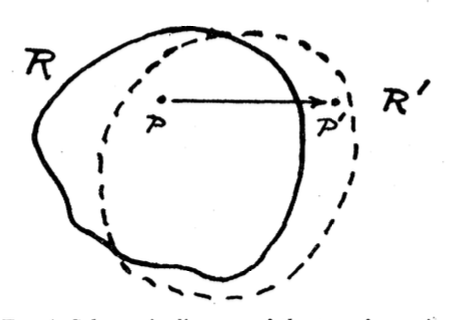
\includegraphics[scale=.5]{fig/img12.png}
\end{figure}
Así,
\begin{align}
  \d S&=\int_{\Omega'}\dd^4x'\L '(x')-\int_\Omega \dd^4x \L (x)\\
\end{align}
donde 
\begin{equation}
  \L(x)=\L (\psi,\partial_\m \psi,x),\qquad \L'(x')=\L' (\psi',\partial'_\m \psi',x')
\end{equation}
y 
\begin{align}
  \d\L(x) &=\L'(x')-\L (x)\implies \L'(x')=\L(x)+\d\L (x)
\end{align}
de manera que
\begin{align}
  \d S&=\int_{\Omega'}\dd^4x'(\L(x)+\d\L (x))-\int_\Omega\dd^4x\L(x)\\
\end{align}
Sabemos que $\dd^4x'$ y $\dd^4x$ se relacionan por $\det$ del Jacobiano,
\begin{align}
  \dd^4x'=J\dd^4x, \qquad \text{con } J=\left|\pdv{x'^\m }{x^\m } \right|
\end{align}
\begin{align}
  J=\left|\pdv{(x^\m +\d x^\m ) }{x^\m } \right|=\left|\pdv{x^\m }{x^\m }+\pdv{\d x^\m }{x^\m }\right|=\left(1+\pdv{\d x^\m }{x^\m }\right)
\end{align}
así,
\begin{align}
  \d S&=\int_{\Omega}\dd^4x\left(1+\pdv{\d x^\m }{x^\m }\right)(\L(x)+\d\L (x))-\int_\Omega\dd^4x\L(x)\\
  &=\int_\Omega\dd^4x \left[\L(x)+\d \L(x)+\pdv{\d x^\m }{x^\m }\L (x)\right]-\int_\Omega\dd^4x\L (x)\\
  &=\int_\Omega\dd^4x\left[\d\L(x)+\pdv{\d x^\m }{x^\m }\L(x)\right]
\end{align}
pero
\begin{equation}
  \d\L(x)=\db\L(x)+\partial_\m \L\d x^\m 
\end{equation}
así
\begin{align}
  \d S&=\int_\Omega\dd^4x\left[\db\L(x)+\partial_\m \L\d x^\m +\partial_\m \d x^\m \L(x)\right]\\
  &=\int_\Omega\dd^4x \left[\db \L(x)+\partial_\m (\L \d x^\m )\right]
\end{align}
pero
\begin{align}
  \db \L(x)=[\L ]\db\psi +\partial_\m \left(\pdv{\L }{(\partial_\m \psi)}\db \psi\right)
\end{align}
luego
\begin{align}
  \d\L &=\db \L +\partial_\m (\L \d x^\m )\\
  &=[\L ]\db\psi+\partial_\m \left(\pdv{\L }{(\partial_\m \psi)}\db \psi+\L \d x^\m\right)\\
  &=[\L ]\db \psi +\partial_\m J^\m 
\end{align}
donde 
\begin{align}
  J^\m &=\pdv{\L }{(\partial_\m \psi)}\db \psi+\L \d x^\m\\
  &=\pdv{\L }{(\partial_\m \psi)}\left(\d \psi-\partial_\n \psi\d x^\n \right)+\L \d x^\m \\
  &=\pdv{\L }{(\partial_\m \psi)}\d\psi -\pdv{\L }{(\partial_\m \psi)}\partial_\n \psi\d x^\n +\L \d x^\m \\
  &=\pdv{\L }{(\partial_\m \psi)}\d\psi +\left(\delta^\m_\n \L -\pdv{\L }{(\partial_\m \psi)}\partial_\n \psi\right)\d x^\n 
\end{align}
Se define,
\begin{align}
  \p^\m &=\pdv{\L }{(\partial_\m \psi)}\\
  T^\m _{~\n }&=\pdv{\L }{(\partial_\m \psi)}\partial_\n \psi-\delta^\m_\n \L 
\end{align}
de manera que
\begin{equation}
 \boxed{ J^\m =\p^\m \delta\psi- T^\m _{~\n }\delta x^\n }
\end{equation}

\subsection{Teoría Electromagnética de Maxwell}
Las ecuaciones de Maxwell vienen dadas por
\begin{align}
  \partial_iE_i &=\frac{\rho}{\epsilon}\label{15.1}\\
  \partial_i B_i&=0\label{15.2}\\
  \epsilon_{ijk}\partial_j E_k&=-\pdv{B_i}{t}\label{15.3}\\
  \epsilon_{ijk}\partial_jB_k&=\m_0 J_i+\m_0\epsilon_0 \pdv{E_i}{t}\label{15.4}
\end{align}
De \eqref{15.2} se tiene que
\begin{equation}
  B_i=\epsilon_{ijk}\partial_j A_k
\end{equation}
\begin{equation}
  \implies \epsilon_{ijk}\partial_j E_k=-\pdv{t}(\epsilon_{ijk}\partial_j A_k)
\end{equation}
\begin{equation}
  \implies \epsilon_{ijl}\partial_j \left(E_k+\pdv{A_k}{t}\right)=0
\end{equation}
\begin{equation}
  \implies E_k=-\partial_k\f -\pdv{A_k}{t}
\end{equation}
Así, las ecuaciones \eqref{15.2} y \eqref{15.3} definen los potenciales electromagnéticos, 
\begin{align}
  \Aboxed{B_i&=\epsilon_{ijk}\partial_j A_k}\\
 \Aboxed{ E_i&=-\partial_i\f -\pdv{A_i}{t}}
\end{align}
La dinámica de estos potenciales vienen determinadas por \eqref{15.1} y \eqref{15.4}.

De \eqref{15.1}
\begin{align}
  \partial_iE_i&=\frac{\rho}{\epsilon_0}\\
  \partial_i\left(-\partial_i\f -\pdv{A_i}{t}\right)&=\frac{\rho}{\epsilon_0}\\
 \Aboxed{ \partial_i\partial_i\f +\pdv{t}\partial_i A_i&=-\frac{\rho}{\epsilon_0}}\label{15.5}
\end{align}
De \eqref{15.4}
\begin{align}
  \epsilon_{ijk}\partial_j(\epsilon_{klm}\partial_l A_m)&=\m_0J_i+\m_0\epsilon_0\pdv{t}\left(-\partial_i\f -\pdv{A_i}{t}\right)\\
  (\delta_{il}\d_{jm}-\d_{im}\d_{jl})\partial_j\partial_l A_m&=\m_0 J_i-\m_0\epsilon_0 \partial_i\pdv{\f}{t}-\m_0\epsilon_0\pdv[2]{A_i}{t}\\
  \partial_j\partial_iA_j-\partial_j\partial_jA_i&=\m_0 J_i-\m_0\epsilon_0\partial_i\pdv{\f }{t}-\m_0\epsilon_0\pdv[2]{A_i}{t}\\
  \partial_j\partial_j A_i-\m_0\epsilon_0\pdv[2]{A_i}{t}&=-\m_0J_i+\partial_i\partial_jA_i+\m_0\epsilon_0 \partial_i\pdv{\f }{t}\\
\Aboxed{ \partial_j\partial_j A_i-\m_0\epsilon_0\pdv[2]{A_i}{t}&=-\m_0J_i+\partial_i\left(\partial_jA_j+\m_0\epsilon_0\pdv{\f }{t}\right)}
\end{align}
De \eqref{15.5}
\begin{align}
  \partial_i\partial_i\f-\m_0\epsilon_0\pdv[2]{\f }{t} &=-\frac{\rho}{\epsilon_0}-\pdv{t}\partial_i A_i--\m_0\epsilon_0\pdv[2]{\f }{t}\\
 \Aboxed{ \partial_i\partial_i\f -\m_0\epsilon_0\pdv[2]{\f }{t}&=-\frac{\rho}{\epsilon_0}-\pdv{t}\left(\partial_iA_i+\m_0\epsilon_0\pdv{\f }{t}\right)}
\end{align}

















































































































% Bibliography

%% [A] Recommended: using JHEP.bst file
%% \bibliographystyle{JHEP}
%% \bibliography{biblio.bib}

%% or
%% [B] Manual formatting (see below)
%% (i) We suggest to always provide author, title and journal data or doi:
%% in short all the informations that clearly identify a document.
%% (ii) please avoid comments such as "For a review'', "For some examples",
%% "and references therein" or move them in the text. In general, please leave only references in the bibliography and move all
%% accessory text in footnotes.
%% (iii) Also, please have only one work for each \bibitem.

\newpage
\bibliographystyle{JHEP}
\bibliography{biblio.bib}
\end{document}
